\graphicspath{ {./figuras/01_reals/} }
\chapter{Números Reais e Hiper-reais}
\label{chp:reals}

O Capítulo~\ref{chp:reals} guia o estudante por um caminho direto até
o ponto onde será possível estudarmos derivadas. As Seções de%
~\ref{sec:realline} até \ref{sec:lines} apresentam uma revisão das
matérias que compõem o pré-cálculo e podem ser omitidas em muitos
cursos de cálculo. A Seção~\ref{sec:hyperrealline} fornece uma
explicação intuitiva para os números hiper-reais e como eles podem
ser usados para encontrar a inclinação de uma curva. Esta seção
não tem nenhum conjunto de problemas e destina-se a formar a base
de uma lição introdutória. O conteúdo principal do Capítulo~\ref{chp:reals}
está nas suas duas útimas seções, \ref{sec:infnumbers} e
\ref{sec:standardparts}. Nestas seções, o estudante aprenderá como
trabalhar com números hiper-reais e, em particular, como calcular
partes padronizadas. Partes padronizadas são usadas no início do próximo
capítulo para encontrar derivadas de funções. As Seções \ref{sec:infnumbers} e 
\ref{sec:standardparts} substituem os capítulos iniciais sobre limites,
encontrados nos textos tradicionais de cálculo.

Para o benefício do estudante interessado, incluímos um Epílogo ao final
do livro que apresenta a teoria por trás deste capítulo.

\section{A Reta Real}
\label{sec:realline}

A familiaridade com o sistema de números reais é um pré-requisito
para este curso. Uma revisão das regras da álgebra para números reais
é dada no apêndice. Por conveniência, estas regras estão também listadas
em uma tabela dentro da primeira capa deste livro. O símbolo
$\setR$ é usado para o conjunto de todos os números reais.
%\tnote{Optamos por divergir da notação original e usar o negrito usado
%em lousa, ou toque duplo (\emph{double-struck}), por ser mais familiar
%aos leitores brasileiros.}
Podemos pensar que os números reais estão dispostos ao longo de uma
reta, com os inteiros marcados a intervalos regulares, como na Figura%
~\ref{fig:realline}. Esta reta é chamada \newdef{reta real}.

\includefig[A reta real.]{realline}

Na matemática dos níveis fundamental e médio, a sistema de números
reais é construído gradualmente em vários estágios. Começando-se
pelos números naturais, continua-se com os inteiros,
racionais e, finalmente, os números reais são construídos. Uma
maneira de se construir o conjunto dos reais é defini-lo
como o conjunto de todos os números que possuem representação
decimal finita ou infinita após a vírgula.

Após a construção dos números reais, é possível demonstrar as
regras familiares de somas, diferenças, produtos, quocientes,
expoentes, raízes e ordem. Neste curso, assumiremos que estas
regras são familiares ao estudante, de tal forma que possamos
proceder o mais rápido possível para o cálculo.

Antes de continuarmos, faremos uma pausa para recapitular dois
pontos de especial importância ao cálculo. Em primeiro lugar,
\emph{a divisão por zero é proibida!} Expressões como
\[
\frac{2}{0}, \hspace{4ex} \frac{0}{0}, \hspace{4ex} 
\frac{x}{0} \hspace{4ex} \frac{5}{1+3-4}
\]
são sempre consideradas como \emph{indefinidas}.

Em segundo lugar, um número real positivo $c$ sempre possui duas
raízes quadradas, $\sqrt{c}$ e $-\sqrt{c}$, onde $\sqrt{c}$ sempre
representará a raiz quadrada positiva. Números reais negativos não
possuem raiz quadrada real. \emph{Para cada número real positivo
$c$, $\sqrt{c}$ é positivo e $\sqrt{-c}$ é indefinido.}

Por outro lado, cada número real possui apenas uma raiz cúbica real.
Se $c > 0$, então $c$ possui a raiz cúbica positiva $\sqrt[3]{c}$, e $-c$
possui a raiz cúbica negativa $\sqrt[3]{-c} = -\sqrt[3]{c}$.

No cálculo, geralmente lidamos com conjuntos de números reais. Por um
conjunto $C$ de números reais, queremos entender qualquer coleção de
números reais, chamados \emph{membros} de $C$, \emph{elementos} de $C$
ou \newdef{pontos} em $C$.

Um conjunto simples, mas importante, é um \newdef{intervalo}. Dados dois
números reais $a$ e $b$ tais que $a < b$, o
\newdef[intervalo!fechado]{intervalo fechado}
$[a, b]$ é definido como o conjunto de todos os números reais $x$
que satisfazem $a \le x$ e $x \le b$, ou de maneira mais concisa,
$a \le x \le b$.
O \newdef[intervalo!aberto]{intervalo aberto} $(a, b)$ é definido como o
conjunto de todos os números reais $x$ que satisfazem $a < x < b$.
Intervalos fechados e abertos estão ilustrados na Figura~\ref{fig:intervals}. 

\widefigure{fig:intervals}
{
	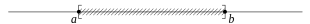
\includegraphics{closedinter}\\
	O intervalo fechado $[a, b]$\\[\baselineskip]
	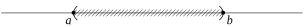
\includegraphics{openinter}\\
	O intervalo aberto $(a, b)$
}

Tanto para o intervalo aberto $(a, b)$, quanto para o intervalo
fechado $[a, b]$, o número $a$ é chamado de
\newdef[extremo!inferior]{extremo inferior},
e $b$ é o \newdef[extremo!superior]{extremo superior}. A diferença entre o
intervalo fechado $[a, b]$ e o intervalo aberto $(a, b)$ é que os extremos $a$
e $b$ são elementos de $[a, b]$, mas não elementos de $(a, b)$. Quando
$a \le x \le b$, dizemos que $x$ está \newdef{entre} $a$ e $b$; quando
$a < x < b$, dizemos que $x$ está \newdef{estritamente entre} $a$ e $b$.

Três outros tipos de conjuntos também são considerados intervalos
abertos: o conjunto $(a, \infty)$ dos números reais $x$ maiores do que $a$;
o conjunto $(-\infty, b)$ dos números reais $x$ menores do que $b$,
e toda a reta real $\setR$. A reta real $\setR$ é, às vezes, denotada
$(-\infty, \infty)$. Os símbolos $\infty$ e $-\infty$, lidos respectivamente
como ``infinito''  e ``menos infinito,'' não representam números reais; eles
só são usados, neste contexto, para indicar intervalos sem extremo
superior ou inferior.

Além dos intervalos fechados e abertos, há um outro tipo de intervalo,
chamado \newdef[intervalo!semiaberto]{intervalo semiaberto}. O conjunto
de todos os números
reais $x$ tais que $a \le x < b$ é um intervalo semiaberto denotado
$[a, b)$. O conjunto de todos os números reais $x$ tais que $a < x \le b$
é também um intervalo semiaberto denotado $(a, b]$.
A Tabela~\ref{tab:intervaltypes} mostra os vários tipos de intervalos.
\tnote{Nesta tradução, optamos por fazer correções sobre as classificações de intervalos neste parágrafo e na tabela.}

\widetable[Tipos de intervalos.]%
{tab:intervaltypes}%
{l @{\hspace{3ex}} l @{\hspace{3ex}} l}%
{
  \hline
  Tipo            & Símbolo         & Definição              \\
  \hline
  Fechado          & $[a, b]$         & $\{ x \in \setR | a \le x \le b \}$ \\
  Fechado          & $[a, \infty)$    & $\{ x \in \setR | a \le x \}$ \\
  Fechado          & $(-\infty, b]$   & $\{ x \in \setR | x \le b \}$ \\
  Aberto           & $(a, b)$         & $\{ x \in \setR | a < x < b \}$ \\
  Aberto           & $(a, \infty)$    & $\{ x \in \setR | a < x \}$ \\
  Aberto           & $(-\infty, b)$   & $\{ x \in \setR | x < b \}$ \\
  Semiaberto       & $(a, b]$         & $\{ x \in \setR | a < x \le b \}$ \\
  Semiaberto       & $[a, b)$         & $\{ x \in \setR | a \le x < b \}$ \\
  Fechado e aberto & $(-\infty, \infty)$ & $\setR$
}

Listamos a seguir alguns outros conjuntos importantes de números reais.

\begin{enumerate}[(1)]
\item O conjunto vazio $\varnothing$, que não possui nenhum elemento.
\item O conjunto finito $\{ a_1, \ldots, a_n \}$, cujos únicos elementos
      são os números $a_1, a_2, \ldots, a_n$.
\item O conjunto $\setR^*$, ou seja, todo $x \in \setR$ tal que $x \ne 0$
\item O conjunto $\setN^* = \{ 1, 2, 3, 4, \ldots \}$ de todos os
      inteiros positivos%
\tnote{O autor usa apenas $\setN$ nesta definição. Optamos por usar
$\setN^*$ para evitar ambiguidade.}
\item O conjunto $\setZ = \{ \ldots, -3, -2, -1, 0, 1, 2, 3, \ldots \}$
      de todos os inteiros
\item O conjunto $\setQ$ de todos os números racionais. Um número
      racional é o quociente $m/n$ onde $m$ e $n$ são inteiros e $n \ne 0$.
\end{enumerate}

Enquanto que números reais correspondem a pontos em uma reta, pares
ordenados de números reais correspondem a pontos em um plano. Esta
correspondência nos dá uma maneira de desenhar gráficos de problemas
no cálculo, e de como traduzir problemas da física para a linguagem do
cálculo. É o ponto de partida da disciplina conhecida como
\newdef{geometria analítica}.

Um \newdef{par ordenado} de números reais, $(a, b)$, é dado
pelo primeiro número $a$ e pelo segundo número $b$. Por exemplo, $(1, 3)$,
$(3, 1)$ e $(1, 1)$ são três pares ordenados
diferentes. Seguindo a tradição, usaremos o mesmo símbolo para o intervalo
aberto $(a, b)$ e para o par ordenado $(a, b)$. Entretanto, o intervalo
aberto e o par ordenado são coisas compleramente diferentes. Será sempre
óbvio pelo contexto se $(a, b)$ significa um intervalo aberto ou
um par ordenado.

Explicaremos como pares ordenados de números reais correspondem a
pontos no plano. Um sistema de \newdef{coordenadas retangulares} no
plano é dado por uma cópia horizontal e uma cópia vertical da reta
real, que se cruzam no zero. A reta horizontal é chamada \newdef{eixo
horizontal} ou \emph{eixo $x$}, enquanto que a reta vertical é chamada
\newdef{eixo vertical} ou \emph{eixo $y$}. O ponto onde os dois
eixos se encontram é chamado \emph{origem} e corresponde ao par
ordenado $(0, 0)$. Considere agora um ponto qualquer $P$ no plano. Uma
reta vertical passando por $P$ cruzará o eixo $x$ em um número real
$x_0$, e uma reta horizontal por $P$ cruzará o eixo $y$ em um número
real $y_0$. O par ordenado $(x_0, y_0)$  obtido desta maneira corresponde
ao ponto $P$. (Ver Figura~\ref{fig:px0y0}) Às vezes chamamos $P$ de ponto
$(x_0, y_0)$, e escreveremos $P(x_0, y_0)$. O número $x_0$ é dito
\newdef{coordenada $x$} de $P$, e $y_0$ é a \newdef{coordenada $y$} de $P$.

Por outro lado, dado um par ordenado $(x_0, y_0)$ de números reais, há um
ponto correspondente $P(x_0, y_0)$ no plano. Determinamos $P(x_0, y_0)$ pelo
ponto de interseção entre a reta vertical que cruza o eixo $x$ em $x_0$
e a reta horizontal que cruza o eixo $y$ em $y_0$. Descrevemos uma
correspondência biunívoca entre todos os pontos no plano e todos os
pares ordenados de números reais.

A partir de agora, simplificaremos as coisas por meio da identidade entre
pontos no plano e pares de números reais, conforme mostramos na Figura%
~\ref{fig:xyisapoint}.

\includefigs{px0y0}{xyisapoint}

\begin{defin}
O \newdef{plano} $(x, y)$ é o conjunto de todos os pares ordenados $(x, y)$
de números reais. A \newdef{origem} é o ponto $(0, 0)$. O \newdef{eixo $x$}
é o conjunto de todos os pontos na forma $(x, 0)$, e o \newdef{eixo $y$} é
o conjunto de todo os pontos na forma $(0, y)$. 
\end{defin}

Os eixos $x$ e $y$ dividem o resto do plano em quatro partes chamadas
\newdef{quadrantes}. Os quadrantes são numerados de I a IV, conforme
Figura~\ref{fig:quadrants}.

Na Figura~\ref{fig:pyththeo}, $P(x_1, y_1)$ e $Q(x_2, y_2)$ são dois
pontos diferentes no plano $(x, y)$. Conforme nos deslocamos de $P$
a $Q$, as coordenadas $x$ e $y$ mudarão por quantidades que
denotaremos $\Delta x$ e $\Delta y$. Logo,
\begin{eqnarray*}
\text{mudança em } x & = \Delta x = & x_2 - x_1, \\
\text{mudança em } y & = \Delta y = & y_2 - y_1.
\end{eqnarray*}
As quantidades $\Delta x$ e $\Delta$ podem ser positivas, negativas ou
zero. Por exemplo, quando $x_2 > x_1$, temos que $\Delta x$ é positivo
e quando $x_2 < x_1$, temos que $\Delta x$ é negativo. Usando $\Delta x$
e $\Delta y$ definimos a noção básica de distância.

\captions{Quadrantes}{}
\includefigs{quadrants}{pyththeo}

\begin{defin}
A \newdef{distância} entre os pontos $P(x_1, y_1)$ e $Q(x_2, y_2)$ é
o valor
\[
  dist\hat{a}ncia(P, Q) = \sqrt{(\Delta x)^2 + (\Delta y)^2}
                        = \sqrt{(x_2 - x_1)^2 + (y_2 - y_1)^2}.
\]
\end{defin}

Elevando os dois lados da fórmula da distância ao quadrado, obtemos
\[
  [dist\hat{a}ncia(P, Q)]^2 = (\Delta x)^2 + (\Delta y)^2.
\]

Também é possível obtermos esta fórmula pelo Teorema de Pitágoras
da geometria: \emph{O quadrado da hipotenusa de um triângulo
retângulo é a soma dos quadrados dos catetos.}

\begin{example}
\label{ex:distance}
Encontre a distância entre $P(7, 2)$ e $Q(4, 6)$
(Veja Figura~\ref{fig:exdist}).
\begin{eqnarray*}
\Delta x = 4 - 7 = -3 &,\phantom{,} & \Delta y = 6 - 2 = 4, \\
 dist\hat{a}ncia(P, Q) & =           & \sqrt{(-3)^2 + 4^2} = 5.
\end{eqnarray*}
\end{example}

\includefig[Cálculo da distância pelo Teorema de Pitágoras.]{exdist}

\begin{defin}[círculo]
O conjunto de todos os pontos no plano que estão a distância $r$ de um ponto
$P$ é chamado o \newdef{círculo} de \newdef{raio} $r$ e \newdef{centro} $P$.
\end{defin}

Usando a fórmula da distância, vemos que o círculo de raio $r$ e centro na
origem (Figura~\ref{fig:locuscirc}) é o lugar geométrico da equação
\[
	x^2 + y^2 = r^2.
\]
O círculo de raio $r$ e centro em $P(h, k)$ (Figura~\ref{fig:locuscirc}) é
o lugar geométrico da equação
\[
	(x-h)^2 + (y-k)^2 = r^2.
\]

\includefig{locuscirc}

Por exemplo, o círculo de raio $3$ e centro em $P(2, -4)$ possui equação
\[
	(x-2)^2 + (y+4)^2 = 9.
\]

\begin{sectionproblems}

%% TODO: conferir se a numeração é igual à do original

\noindent Nos problemas de 1 a 6, encontre a distância entre
          os pontos $P$ e $Q$.

\twoexer{$P(2, 9),   Q(-1, 13)$}%
        {$P(1, -2),  Q( 2, 10)$}

\twoexer{$P(0, 0),   Q(-2, -3)$}%
        {$P(-1, -1), Q( 4, 4)$}

\twoexer{$P(6, -1),  Q(-7, 1)$}%
        {$P(5, 10),  Q( 9, 10)$}

\noindent Esboce os círculos dados nos problemas de 7 a 12.

\twoexer{$x^2+y^2 = 4$}%
        {$x^2 + y^2 = \frac{1}{4}$}

\twoexer{$(x - 1)^2 + (y + 2)^2 = 1$}%
        {$(x+2)^2 + (y+3)^2 = 9$}

\twoexer{$(x - 1)^2 + (y - 1)^2 = 2$}%
        {$(x+3)^2 + (y-4)^2 = 25$}

\exer{Encontre a equação do círculo de raio $2$ e centro $(3, 0)$.}

\exer{Encontre a equação do círculo de raio $\sqrt{3}$ e centro $(-1, -2)$.}

\hardex{Há dois círculos de raio $2$ que possuem centro na reta
        $x = 1$ e que passam pela origem. Encontre suas equações.}

\hardex{Encontre a equação do círculo que passa pelos pontos
        $(0, 0)$, $(0, 1)$ e $(2, 0)$.}

\hardex{Encontre a equação do círculo tal que o segmento de reta
        entre $(-1, 0)$ e $(5, 8)$ seja seu diâmetro.}

\end{sectionproblems}

\section{Funções de Números Reais}
\label{sec:funcreal}

As próximas duas seções tratam apenas de números reais. O cálculo
lida com problemas nos quais uma quantidade depende de uma ou mais
outras quantidades. Por exemplo, a área do círculo depende de seu
raio. O comprimento de um dia depende tanto da latitude quanto da
data. O preço de um objeto depende da oferta e da demanda. A maneira
pela qual uma quantidade depende de outra(s) pode ser descrita
matematicamente por uma função de uma ou mais variáveis.

\begin{defin}
Uma \newdef{função real de uma variável} é um conjunto $f$ de pares
ordenados de números reais tal que, para cada número real $a$, uma
das seguintes coisas acontece:

\begin{enumerate}[(i)]
\item Há exatamente um número real $b$ para o qual o par ordenado $(a, b)$
é um membro de $f$. Neste caso, dizemos que $f(a)$ é definido e
escrevemos $f(a) = b$. O número $b$ é chamado o valor de $f$ em $a$.
\item Não há nenhum número real $b$ para o qual o par ordenado $(a, b)$
é um membro de $f$. Neste caso, dizemos que $f(a)$ é indefinido.
\end{enumerate}
\end{defin}

Logo, $f(a) = b$ significa que o par ordenado $(a, b)$ é um elemento
de $f$.

Uma maneira de visualizar uma função é imaginar uma caixa preta, a qual
rotularemos $f$, conforme a Figura~\ref{fig:funcbox}. Dentro da caixa há
alguma máquina, a qual não podemos ver. Em ambos os lados da caixa,
esquerdo e direito, há uma cópia da reta real, chamadas reta de entrada
e reta de saída, respectivamente. Toda vez que indicarmos um número $a$
na reta de entrada, ou um ponto $b$ será marcado na reta de saída para
nos dizer que $f(a) = b$, ou nada irá acontecer no caso em que $f(a)$
é indefinido.

\includefig{funcbox}

Uma segunda maneira de visualizar uma função é desenhando o seu gráfico.
O \newdef{gráfico} de uma função real $f$ de uma variável é o conjunto de
todos os pontos no plano $P(x, y)$ tais que $y = f(x)$. Para desenhar o
gráfico, localizamos o valor de $x$ no eixo horizontal (eixo $x$) e
o valor de $f(x)$ no eixo vertical (eixo $y$). Como podemos dizer se
um conjunto de pontos no plano é o gráfico de alguma função? Lendo-se
novamente a definição de uma função, temos uma resposta.

Um conjunto $C$ de pontos no plano é o gráfico de alguma função $f$ se,
e somente se, para cada reta vertical do plano uma das seguintes
condições é verdadeira:
\begin{enumerate}[(1)]
\item Exatamente um ponto na reta pertence ao conjunto $C$.
\item Nenhum ponto na reta pertence ao conjunto $C$.
\end{enumerate}

Uma reta vertical cruzando o eixo $x$ em um ponto $a$ irá encontrar
o conjunto $C$ em exatamente um ponto $(a, b)$ se $f(a)$ está definido
e $f(a) = b$, e a reta não encontrará o conjunto $C$ de nenhuma forma
se $f(a)$ for indefinido. Experimente usar essa regra para os conjuntos
de pontos mostrados na Figura~\ref{fig:grafrule}.

\includefig{grafrule}

Os exemplos~\ref{ex:funcquad} e \ref{ex:funcrec} ilustram algumas funções
reais de uma variável. Cada função será
descrita de duas maneiras: a abordagem por caixa preta, onde uma regra é
dada para se encontrar o valor da função para cada número real, e o método
pelo gráfico, onde uma equação é dada para o gráfico da função.

\begin{example}\label{ex:funcquad}
A \newdef[função!quadrática]{função quadrática}.

A função quadrática é definida pela regra
\[
  f(x) = x^2
\]
para cada número real $x$. O valor de $f(a)$ é obtido tomando-se o
quadrado de $a$. Por exemplo, os valores de $f(0)$, $f(2)$, $f(-3)$,
$f(r)$ e $f(r+1)$ são
\begin{eqnarray*}
   f(0) = 0, && \hspace{0.1\textwidth} f(2) = 4,
  \hspace{0.1\textwidth} f(-3) = 9,  \\
 f(r) = r^2, && \hspace{0.1\textwidth} f(r+1) = r^2 + 2r + 1.
\end{eqnarray*}
O gráfico da função quadrática é a parábola com equação $y = x^2$.
O gráfico de $y = x^2$, com vários pontos destacados, é mostrado
na Figura~\ref{fig:exparabola}.
\end{example}

\includefigs{exparabola}{exreciprocal}

\begin{example}\label{ex:funcrec}
A \newdef[função!recíproca]{função recíproca}.

A função recíproca é definida pela regra
\[
  g(x) = \frac{1}{x},
\]
$g(x)$ é definido para todo $x$ não nulo, mas é indefinido para
$x = 0$. Encontre os seguintes valores, se estiverem definidos:
$g(0)$, $g(2)$, $g\left(-\frac{1}{3}\right)$,
$g\left(\frac{7}{4}\right)$, $g(r+1)$.
\begin{eqnarray*}
  g(0) \text{ é indefinido}, & \SPC & g(2) = \frac{1}{2}, \SPC g\left(-\frac{1}{3}\right) = -3, \\
  g\left(\frac{7}{4}\right) = \frac{4}{7}, & & g(r+1) = \frac{1}{r + 1} \text{ se } r \ne -1.
\end{eqnarray*}
O gráfico da função recíproca possui equação $y = \frac{1}{x}$. Esta
equação também pode ser escrita na forma $x y = 1$. O gráfico é
mostrado na Figura~\ref{fig:exreciprocal}.
\end{example}

Nos exemplos~\ref{ex:funcquad} e~\ref{ex:funcrec} usamos as variáveis
$x$ e $y$ para descrever uma função. Uma \newdef{variável} é uma
letra que toma o significado de um número real arbitrário; isto é,
que ``varia'' sobre a reta real. Na equação $y = x^2$ o valor de $y$
depende do valor de $x$; por esta razão, dizemos que $x$ é a
\newdef[variável!independente]{variável independente} e $y$ é a
\newdef[variável!dependente]{variável dependente} da equação.

Ao descrever uma função, nem sempre usamos $x$ e $y$;
às vezes outras variáveis são mais convenientes, especialmente
em problemas envolvendo várias funções. A variável $t$ é comumente
usada para denotar o tempo.

É importante fazer a distrinção entre os símbolos $f$ e 
$f(x)$. O símbolo $f$ denomina a \emph{função}, enquanto que
$f(x)$ é chamado de \emph{termo} e denota o valor da função
em $x$. A necessidade desta distinção é ilustrada no exemplo~%
\ref{ex:distinctfunc}

\begin{example}\label{ex:distinctfunc}
Seja $h$ a função dada pela regra
\[
  h(t) = t^3 + 1.
\]
Note que $t$ é uma variável, $h$ uma função e $h(t)$ um termo.
As seguintes expressões também são termos: $h\left(\frac{1}{2}\right)$,
$h(x)$, $h(t^3)$, $h(t^3) + 1$, $h(t^3+1)$, $h(x) - h(t)$, $h(t + \Delta t)$,
$h(t+\Delta t) - h(t)$. Encontre os valores para cada um desses termos.

% hausen: substituí abaixo 1 1/8 por 9/8
Os valores podem ser encontrados por uma substituição cautelosa.
\begin{eqnarray*}
  h\left(\frac{1}{2}\right) & = & \left(\frac{1}{2}\right)^3 + 1 = \frac{9}{8}. \\
  h(x) & = & x^3 + 1. \\
  h(t^3) & = & \left(t^3\right)^3 + 1 = t^9 + 1. \\
  h(t^3) + 1 & = & \left[ \left( t^3 \right)^3 + 1 \right] + 1 = t^9 + 2. \\
  h(t^3 +  1) & = & \left( t^3 + 1 \right)^3 + 1 = t^9 + 3t^6 + 3t^3 + 2. \\
  h(x) - h(t) & = & \left[ x^3 + 1 \right] - \left[ t^3 + 1 \right] =
                    x^3 - t^3. \\
  h(t + \Delta t) & = & (t + \Delta t)^3 + 1 = t^3 + 3t^2 \Delta t +
                        3t \Delta t^2 + \Delta t^3 + 1. \\
  h(t + \Delta t) - h(t) & = &
                \left[ (t + \Delta t)^3 + 1 \right] -
                \left[ t^3 + 1 \right] \\
                         & = &
                \left[ t^3 + 3t^2 \Delta t +
                       3t \Delta t^2 + \Delta t^3 + 1 \right] -
                \left[ t^3 + 1 \right] \\
                         & = & 3t^2 \Delta t + 3t \Delta t^2 + \Delta t^3.
\end{eqnarray*}
O gráfico de $h$ é dado pela equação $x = t^3 + 1$. Nesta equação,
$t$ é a variável independente e $x$ é a variável dependente. Na Figura~%
\ref{fig:excubic}, os cinco pontos
\[
\textstyle
  h(-1) = 0, \SPC h\left(-\frac{1}{2}\right) = \frac{7}{8}, \SPC
% hausen: substituí abaixo 1 1/8 por 9/8
  h(0) = 1, \SPC h\left(\frac{1}{2}\right) = \frac{9}{8}, \SPC
  h(1) = 2
\]
são marcados e o gráfico é desenhado.
\end{example}

\includefig{excubic}

\begin{defin}
O \newdef{domínio} de uma função real $f$ de uma variável é o conjunto
de todos os números reais $x$ para os quais $f(x)$ está definido.

A \newdef{imagem} de $f$ é o conjunto de todo os valores $f(x)$
tais que $x$ está no domínio de $f$.
\end{defin}

\begin{examplecont}{ex:funcquad}
O domínio da função quadrática é o conjunto $\setR$ de todos os números
reais. A imagem é o intervalo $[0, \infty)$ de todos os reais não negativos.
\end{examplecont}

\begin{examplecont}{ex:funcrec}
Tanto o domínio quanto a imagem da função recíproca são iguais ao
conjunto de todos os números reais $x$ que satisfazem $x \ne 0$.
\end{examplecont}

Quando uma função é descrita por uma regra, é entendido que o domínio
é o conjunto de todos os números reais para os quais aquela regra faz
sentido.

\begin{examplecont}{ex:distinctfunc}
A função $h$ dada pela regra
\[
  h(t) = t^3 + 1
\]
possui toda a reta real como domínio e como imagem.
\end{examplecont}

\begin{example}
\label{ex:sqrt1x2}
Seja $f$ a função dada pela regra
\[
  f(x) = \sqrt{1 - x^2}.
\]
Ou seja, $f(x)$ é a raiz quadrada positiva de $1 - x^2$. O domínio
de $f$ é o intervalo fechado $[-1, 1]$. A imagem de $f$ é $[0, 1]$.

Por exemplo,
\begin{eqnarray*}
\textstyle
  f(-2) \text{ é indefinido}, \SPC f(-1) & = & 0, \SPC f(0) = 1, \\
  f\left(\frac{1}{2}\right) = \sqrt{\frac{3}{4}}, \SPC f(1) & = & 0,
                                   \SPC f(2) \text{ é indefinido}.
\end{eqnarray*}

O gráfico de $f$ é dado pela equação $y = \sqrt{1-x^2}$.

A equação também pode ser escrita na forma
\[
  x^2 + y^2 = 1, y \ge 0.
\]

O gráfico é apenas a metade superior do semicírculo unitário, mostrado
na Figura~\ref{fig:sqrt1x2}.
\end{example}

\includefig{sqrt1x2}

Às vezes uma função é descrita pela menção explícita ao domínio, além
de uma regra.

\begin{example}
Seja $g$ uma função cujo domínio é o intervalo fechado $[1, 2]$ e com
a regra
\[
  g(x) = x^2.
\]
O domínio e a regra podem ser escritos de maneira concisa com uma
equação e desigualdades,
\[
  g(x) = x^2, \SPC 1 \le x \le 2.
\]
\begin{eqnarray*}
   & g(0) \text{ é indefinido} \SPC g(1) = 1 & \\
   & g(2) = 4 \SPC g(3) \text{ é indefinido} &
\end{eqnarray*}
O gráfico é definido pelas fórmulas
\[
   y = x^2, \SPC 1 \le x \le 2
\]
e está desenhado na Figura~\ref{fig:truncparabola}
\end{example}

\includefigs{truncparabola}{constantfunc}

Algumas funções especialmente importantes são as \emph{funções
constantes}, a \emph{função identidade} e a \emph{função valor
absoluto}.

Um número real por vezes é chamado de \newdef{constante}. Este
nome é usado para enfatizar a diferença entre um número real
fixo e uma variável.

Para um número real $c$ dado, a função $f$ com a regra
\[
  f(x) = c
\]
é chamada de \newdef[função!constante]{função constante} com
valor $c$. Seu domínio é $\setR$ e sua imagem é $\{c\}$.

\begin{example}
\label{ex:constantfunc}
A função constante com valor $5$ é descrita pela regra $f(x) = 5.$

Logo \SPC $f(0) = 5$, \SPC $f(-3) = 5$, \SPC $f(\fnum{1000000}) = 5$.

O gráfico (Figura~\ref{fig:constantfunc}) da função constante com
valor 5 é dado pela equação $y=5$.
\end{example}

\begin{example}
\label{ex:identityfunc}
A função $f$ dada pela regra
\[
  f(x) = x
\]
é chamada de \newdef[função!identidade]{função identidade}.

O gráfico (Figura~\ref{fig:identityfunc}) da função identidade é a
reta com equação $y=x$.
\end{example}

\includefig{identityfunc}

A \emph{função valor absoluto} é definida por uma regra que é
dividida em dois casos.

\begin{defin}
\index{valor absoluto}\index{módulo}
A \newdef[função!valor absoluto]{função valor absoluto} $|\SPC|$,
por vezes também denominada \newdef[função!módulo]{função módulo}, é
definida por
\[
  |x| = \left\{
        \begin{array}{rl}
         x & \SPC \text{se } x \ge 0,\\
        -x & \SPC \text{se } x < 0.
        \end{array}
        \right.
\]
\end{defin}

O valor absoluto de $x$ dá a distância entre $x$ e $0$. Ele
é sempre positivo ou zero. Por exemplo,
\[
  |3| = 3, \SPC |-3| = 3, \SPC |0| = 0.
\]
O domínio da função valor absoluto é toda a reta real $\setR$,
enquanto que a sua imagem é o intervalo $[0, \infty)$.

A função valor absoluto também pode ser descrita pela regra
\[
  |x| = \sqrt{x^2}.
\]
Seu gráfico é dado pela equação $y = \sqrt{x^2}$. O gráfico é
na forma de um ``V,'' conforme mostrado na Figura~\ref{fig:absfunc}.

\includefig{absfunc}

Se $a$ e $b$ são dois pontos na reta real, então da definição
de $|x|$ podemos ver que
\[
  |a - b| = \left\{
            \begin{array}{r l}
              a - b & \SPC \text{se } a \ge b, \\
              b - a & \SPC \text{se } b > a.
            \end{array}
            \right.
\]
Logo, $|a-b|$ é a diferença entre o maior e o menor
dos dois números. Em outras palavras, $|a-b|$ é a
\emph{distância} entre os pontos $a$ e $b$ na reta real,
como ilustrado na Figura~\ref{fig:distAB}.

\includefig{distAB}

Por exemplo, $|2-5| = 3$, $|4 - (-4)| = 8$. Eis aqui alguns
fatos úteis sobre valores absolutos.

\begin{theorem}
\label{theo:absvalues}
Sejam $a$ e $b$ números reais.
\begin{enumerate}[(i)]
  \item $|-a| = |a|$.
  \item $|ab| = |a|\cdot|b|$.
  \item Se $b \ne 0$, $\displaystyle\left|\frac{a}{b}\right| = \frac{|a|}{|b|}$.
\end{enumerate}
\end{theorem}

\begin{proof}
Usaremos a equação $|x| = \sqrt{x^2}$.
\begin{enumerate}[(i)]
  \item $|-a| = \sqrt{(-a)^2} = \sqrt{a^2} = |a|.$
  \item $|ab| = \sqrt{(ab)^2} = \sqrt{a^2b^ 2} = \sqrt{a^2}\sqrt{b^2}
         = |a|\cdot|b|.$
  \item Prova similar a (ii).
\end{enumerate}
\end{proof}

\begin{warning}
A equação $|a + b| = |a|+|b|$ é \emph{falsa} em geral. Por exemplo,
$|2 + (-3)| = 1$, enquanto que $|2| + |(-3)| = 5$. Ela será verdadeira
quando ambos os números forem positivos, quando ambos forem negativos,
ou quando um deles for nulo.
\end{warning}

Funções emergem em uma grande variedade de situações. Temos aqui
alguns exemplos.

\emph{Geometria:}
\begin{eqnarray*}
     \pi r^2 & = & \text{área de um círculo com raio } r \\
   4 \pi r^2 & = & \text{área da superfície de uma esfera com raio } r \\
\textstyle
   \frac{4}{3}\pi r^3 & = & \text{volume de uma esfera com raio } r \\
   \sen \theta & = & \text{o seno de um ângulo } \theta
\end{eqnarray*}

\emph{Física:}
\begin{eqnarray*}
  s(t) & = & \text{distância percorrida por uma partícula do instante } 0 \text{ até } t \\
  v(t) & = & \text{velocidade de uma partícula no instante } t \\
  a(t) & = & \text{aceletação de uma partícula no instante } t \\
  p(y) & = & \text{pressão da água à profundidade } y \text{ abaixo da superfície} \\
     C & = &\textstyle \frac{5}{9}(F - 32) = \text{ temperatura em graus Celsius como}\\
       &   & \text{função da temperatura em graus Fahrenheit}
\end{eqnarray*}

\emph{Economia:}
\begin{eqnarray*}
  f(t) & = & \text{população no instante } t \\
  p(t) & = & \text{preço de um produto no instante } t \\
  c(x) & = & \text{custo de } x \text{ itens de um produto} \\
  D(p) & = & \text{demanda de um produto a um preço } p \text{, i. e.,} \\
       &   & \text{a quantidade que pode ser vendida a preço } p
\end{eqnarray*}

Funções de duas ou mais variáveis podem ser tratadas de maneira
similar. A seguir temos a definição precisa de uma função de
duas variáveis.

\begin{defin}
Uma \newdef{função real de duas variáveis} é um conjunto $f$ de
triplas ordenadas de números reais tal que, para cada par ordenado
de números reais $(a, b)$, uma das seguintes coisas acontece:
\begin{enumerate}[(i)]
\item Há exatamente um número real $c$ para o qual a tripla
      ordenada $(a, b, c)$ é um membro de $f$. Neste caso, $f(a, b)$
      é definido e escrevemos:
\[
  f(a, b) = c.
\]
\item Não há nenhum número real $c$ para o qual a tripla
      ordenada $(a, b, c)$ é um membro de $f$. Neste caso,
      dizemos que $f(a, b)$ é indefinido.
\end{enumerate}
\end{defin}

Se $f$ é uma função real de duas variáveis, então o valor
de $f(x, y)$ depende tanto do valor de $x$ quanto do valor
de $y$ quando $f(x, y)$ está definido.

Uma função real $f$ de duas variáveis pode ser visualizada
como uma caixa preta com \emph{duas} retas de entrada e uma
reta de saída, como na Figura~\ref{fig:func2box}.

\includefig{func2box}

O \emph{domínio} de uma função real $f$ de duas variáveis é
o conjunto de todos os pares de números reais $(x, y)$ para os
quais $f(x, y)$ está definido.

Os exemplos mais importantes de funções reais de duas variáveis
são as funções soma, diferença, produto e quociente:
\begin{eqnarray*}
  f(x, y) = x+y, & \SPC & f(x, y) = xy, \\
  f(x, y) = x-y, & \SPC & \textstyle f(x, y) = \frac{x}{y},
\end{eqnarray*}

As funções soma, diferença e produto possuem o plano inteiro
como domínio. O domínio da função quociente é o conjunto de
todos os pares ordenados $(x, y)$ tais que $y \ne 0$.

Temos aqui alguns exemplos de funções de duas ou mais variáveis
que aparecem em aplicações.

\emph{Geometria:}
\begin{eqnarray*}
  ab & = & \text{área de um retângulo com lados $a$, $b$} \\
 abc & = & \text{volume do sólido retangular com arestas $a$, $b$, $c$} \\
\textstyle
\frac{1}{2}bh & = & \text{área de um triângulo com base $b$ e altura $h$} \\
\pi r^2 h & = & \text{volume de um cilindro com base circular de raio $r$ e altura $h$} \\
\textstyle
\frac{1}{3} \pi r^2 h & = & \text{volume de um cone com base circular
                            de raio $r$ e altura $h$} \\
\textstyle
\sqrt{x^2 + y^2} & = & \text{distância da origem ao ponto } (x, y)
\end{eqnarray*}

\emph{Física:}
\begin{eqnarray*}
 F = ma & = & \text{força requerida para dar à massa $m$ a aceleração $a$} \\
\rho(x, y, z) & = & \text{densidade de um objeto tridimensional no ponto $(x, y, z)$} \\
 F = G m_1 m_2 / s^2 & = &
    \text{força gravitacional entre objetos com massas $m_1$ e $m_2$} \\
                     &   &
    \text{a uma distância $s$}\\
 m = \frac{m_0}{\sqrt{1-v^2/c^2}} & = &
    \text{massa relativística de um objeto com massa $m_0$ em repouso} \\[-8pt]
                                  &   &
    \text{e velocidade $v$}
\end{eqnarray*}

\emph{Economia:}
\begin{eqnarray*}
 c(x, y) & = & \text{custo de $x$ itens de um produto e $y$ itens de outro} \\
         &   & \text{produto} \\
 D_1(p_1, p_2) & = & \text{demanda para produto 1, quando produto 1 tem preço $p_1$}\\
              &   & \text{e produto 2 tem preço $p_2$}
\end{eqnarray*}

\begin{sectionproblems}

Para cada um dos problemas a seguir (Problemas 1--8), faça uma tabela
mostrando o valor de $f(x)$ quando $x = -1, -\frac{1}{2}, 0, \frac{1}{2}, 1$.
Coloque um * onde $f(x)$ é indefinido.\\

Exemplo:
$\displaystyle f(x) = \frac{1}{x}$%
\SPC\SPC\SPC%
\begin{tabular}{c @{\SPC} | @{\SPC} c @{\SPC} c @{\SPC} c @{\SPC} c @{\SPC} c}
   $x$ & $-1$ & $-\frac{1}{2}$ & $0$ & $\frac{1}{2}$ & $1$ \\
\hline
$f(x)$ & $-1$ &     $-2$       &  *  &      $2$      & $1$
\end{tabular}\\

\twoexer{$f(x) = x/3$}%
        {$f(x) = 3$}
\twoexer{$f(x) = 3x^3 - 5x^2 + 2$}%
        {$f(x) = 1/(x-1)$}
\twoexer{$f(x) = \sqrt{-x}$}%
        {$f(x) = |x|$}
\exer{$f(x) = \left|x-\frac{1}{2}\right| + \left|x+\frac{1}{2}\right|$}
\exer{$f(x) = \sqrt{x^2-1}$}
\exer{O conjunto de pares ordenados $\{ (3, 2), (0, 1), (4, 2) \}$ é uma função?}
\exer{O conjunto de pares ordenados $\{ (0, 2), (3, 6), (3, 4) \}$ é uma função?}
\exer{Seja $f$ a função tal que $f(x) = 1 + x + x^2$. Determine
      $f(2)$, $f(t)$, $f(t + \Delta t)$, $f(1+t+t^2)$, $f(g(t))$.}
\exer{Seja $f(x) = 1/x$. Determine $f(t), f(t+\Delta t), f(t^2),
      f(1/t), f(g(t))$.}
\exer{Seja $f(x) = x\sqrt{x}$. Determine $f(t), f(t+\Delta t), f(t^2),
      f(\sqrt{t}), f(g(t))$.}
\exer{Seja $f(x) = ax+b$. Determine $f(ct+d), f(t^2),
      f(1/t), f(t/a), f(g(t))$.}

Para cada uma das funções seguintes (Problemas 15--20), determine
$f(x + \Delta x) - f(x)$.

\twoexer{$f(x) = 4x + 1$}%
        {$f(x) = x^2 - x$}
\twoexer{$f(x) = x^{-2}$}%
        {$f(x) = x^4$}
\twoexer{$f(x) = \sqrt{x}$}%
        {$f(x) = 4$}

Determine o domínio das funções abaixo (Problemas 21--25)

\twoexer{$f(x) = 1/(x^2 - 1)$}%
        {$f(z) = \sqrt{z^2 - 1}$}

\twoexer{$f(x) = \sqrt{x}$}%
        {$f(t) = \sqrt{|t|}$}

\exer{$f(x) = 1/\sqrt{1-x^2}$}

\hardex{
  Demonstre que:
  \begin{enumerate}[(i)]
    \item se $a$ e $b$ têm o mesmo sinal, então $|a+b| = |a|+|b|$.
    \item se $a$ e $b$ têm sinais opostos, então $|a+b| < |a|+|b|$.
  \end{enumerate}
}

\end{sectionproblems}

\section{Retas}
\label{sec:lines}

\begin{defin}
Seja $P(x_0, y_0)$ um ponto e $m$ um número real. A \newdef{linha reta},
ou apenas \newdef{reta}, por $P$
com inclinação $m$ é o conjunto de todos os pontos $Q(x, y)$ tais que
\[
  y - y_0 = m(x - x_0).
\]
Esta equação é chamada de \newdef[equação!por ponto e inclinação]{equação
por ponto e inclinação} %
\index{forma!por ponto e inclinação}%
da reta.
(Veja figura~\ref{fig:pointslope})
A \newdef[reta!vertical]{reta vertical} por $P$ é o conjunto de todos os
pontos $Q(x, y)$ tais que $x = x_0$. Retas verticais não possuem valor
real para a sua inclinação.
\end{defin}

\includefig{pointslope}

A inclinação é a medida da direção que uma reta segue. A Figura%
~\ref{fig:exslopes} mostra retas com inclinações: zero; positiva;
e negativa.

\widefigure{fig:exslopes}%
{
\hfill
\begin{picture}(50,62)(0,-12)
\thicklines
\put(0,30){\line(1,0){50}}
\put(0,0){Inclinação = 0}
\end{picture}%
\hfill%
\begin{picture}(50,62)(0,-12)
\thicklines
\put(0,15){\line(2,1){50}}
\put(0,0){Inclinação $>$ 0}
\end{picture}%
\hfill%
\begin{picture}(50,62)(0,-12)
\thicklines
\put(0,40){\line(2,-1){50}}
\put(0,0){Inclinação $<$ 0}
\end{picture}%
\hfill%
\begin{picture}(50,62)(0,-12)
\thicklines
\put(25,10){\line(0,1){40}}
\put(12,0){Vertical}
\put(0,-12){sem inclinação}
\end{picture}
\hspace*{\fill}
}

A reta que cruza o eixo $y$ no ponto $(0, b)$ e possui inclinação $m$
tem a equação simples
\[
  y = mx + b.
\]
Esta é chamada a forma %
\newdef[equação!por inclinação e intercepto]{por inclinação e intercepto} %
\index{forma!por inclinação e intercepto}%
da equação de uma reta. Podemos obtê-la a partir da forma por
ponto e inclinação fazendo-se $x_0 = 0$ e $y_0 = b$.

\begin{example}
A reta pelo ponto $P(-1, 2)$ com inclinação $m = - \frac{1}{2}$
(Figura~\ref{fig:expointslope}) tem a seguinte equação por
ponto e inclinação
\[
  y-2 = (x - (-1))\cdot(-\frac{1}{2}), \SPC \text{ou}
  \SPC y-1 = -\frac{1}{2}(x+1).
\]
A equação por inclinação e intercepto é
% hausen: substituí a fração mista por imprópria 1 1/2 -> 3/2
\[
  y = -\frac{1}{2}x + \frac{3}{2}
\]
\end{example}

\includefig{expointslope}

Passaremos à descrição das funções cujos gráficos são retas não verticais.

\begin{defin}
Uma \newdef[função!linear]{função linear} é uma função $f$ da forma
\[
  f(x) = mx+b,
\]
onde $m$ e $b$ são constantes.
\end{defin}

O gráfico de uma função linear é apenas a reta cuja equação por
inclinação e intercepto é
\[
  y = mx+b,
\]
ou seja, a reta por $(0, b)$ com inclinação $m$.

Se dois pontos em uma reta são conhecidos, a inclinação pode ser
determinada da seguinte maneira.

\begin{theorem}
\label{theo:slope}
Suponha que uma reta $L$ passa por dois pontos distintos $P(x_1, y_1)$
e $Q(x_2, y_2)$. Se $x_1 = x_2$ e $y_1 \ne y_2$, então a reta é vertical.
Se $x_1 \ne x_2$ e $y_1 \ne y_2$, então a inclinação da reta $L$ é
igual à mudança em $y$ dividida pela mudança em $x$, ou seja,
\[
  m = \frac{\Delta y}{\Delta x} = \frac{y_2 - y_2}{x_2 - x_1}.
\]
\end{theorem}

\begin{proof}
Suponha que $x_1 \ne x_2$ e $y_1 \ne y_2$, logo $L$ não é vertical. Seja
$m$ a inclinação de $L$. A reta $L$ terá a seguinte fórmula por ponto e
inclinação
\[
  y - y_1 = m (x-x_1).
\]
Substituindo-se $y_2$ por $y$ e $x_2$ por $x$, vemos que
$m = (y_2 - y_1)/(x_2 - x_1)$.
\end{proof}

O Teorema~\ref{theo:slope} mostra por que a inclinação de uma
reta é a medida de sua direção. Às vezes $\Delta x$ é denominado
\newdef{deslocamento} e $\Delta y$ é denominado
\newdef{elevação}. Portanto, a inclinação é igual à elevação
dividida pelo deslocamento. Uma grande inclinação positiva
implica que a reta está se elevando rapidamente à direita,
e uma pequena inclinação positiva indica que a reta se eleva
lentamente à direita. Uma inclinação negativa indica que a
reta desce quando caminhamos para a direita. Estes casos estão
ilustrados na Figura~\ref{fig:slopeanalysis}.

\includefig{slopeanalysis}

% XXX: há um erro na página 18 do livro do Keisler, no parágrafo
%      abaixo. P(x1, y2) corrigido para P(x1, y1) na versão em português
Há exatamente uma reta $L$ que passa por dois pontos distintos
$P(x_1, y_1)$ e $Q(x_2, y_2)$. Se $x_1 \ne x_2$, vemos pelo
Teorema~\ref{theo:slope} que $L$ tem equação
\[
  y - y_1 = \left( \frac{y_2 - y_1}{x_2 - x_1} \right) (x - x_1).
\]
Esta é chamada a \newdef[equação!da reta por dois pontos]%
{equação da reta por dois pontos}.

\begin{example}
Dados $P(3, 1)$ e $Q(1, 4)$, determine as mudanças em $x$ e $y$,
a inclinação e a equação da reta por $P$ e $Q$. (Veja
Figura~\ref{fig:exslope2}.)
\[
  \Delta x = 1 - 3 = -2, \SPC \Delta y = 4 - 1 = 3.
\]
A reta por $P$ e $Q$ tem inclinação $\Delta y / \Delta x = -\frac{3}{2}$,
e sua equação é
\[
  y - 1 = -\frac{3}{2}(x-3).
\]
\end{example}

\includefig{exslope2}

\begin{example}
Dados $P(1, -1)$ e $Q(1, 2)$ como na Figura~\ref{fig:exslope3},
\[
  \Delta x = 1 - 1 = 0, \SPC \Delta y = 2 - (-1) = 3.
\]
A reta por $P$ e $Q$ é a reta vertical $x = 1$.
\end{example}

\includefig{exslope3}

\begin{example}
Uma partícula se move ao longo do eixo $y$ com velocidade
constante. No instante $t=0$ segundo, ela está na posição
$y = 3$ metros. No instante $t = 2$ segundos, ela está na
posição $y = 11$ metros. Determine a velocidade e a
equação para o movimento.

% XXX: adicionei "média" após velocidade, e refraseei o
%      parágrafo
A velocidade média é definida como a distância percorrida dividida
pelo tempo transcorrido. Como a velocidade é constante:
\[
  v = \frac{\Delta y}{\Delta x} = \frac{11-3}{2-0} = 4 \text{m/s}.
\]

Se o movimento da partícula for desenhado no plano $(t, y)$
conforme a Figura~\ref{fig:exslope4}, o resultado é uma reta
pelos pontos $P(0, 3)$ e $Q(2, 11)$. A velocidade média,
sendo a razão de $\Delta y$ para $\Delta x$, é apenas a
inclinação desta reta. A reta possui equação
\[
  y - 3 = 4t
\]
\end{example}

\includefig{exslope4}

Suponha que uma partícula se deslocando com velocidade 
constante está sobre o ponto $y = y_1$ no instante
$t = t_1$, e sobre o ponto $y = y_2$ no instante $t = t_2$.
Então a velocidade é $v = \Delta y / \Delta t$. O movimento
da partícula traçado no plano $(t, y)$ é a reta passando pelos
dois pontos $(t_1, y_1)$ e $(t_2, y_2)$, e a velocidade é a
inclinação desta linha.

Uma equação da forma
\[
  Ax + By + C = 0,
\]
onde $A$ e $B$ não são ambos nulos é chamada
\newdef[equação!linear]{equação linear}. A razão para
este nome será explicada no Teorema~\ref{theo:lineareq}.

\begin{theorem}\label{theo:lineareq}
Toda equação linear define uma linha reta.
\end{theorem}

\begin{proof}
\begin{caseanalysis}
\item $B = 0$. A equação $Ax + C = 0$ pode ser resolvida
para $x$, logo $x = -C/A$. Isto define uma reta vertical.

\item $B \ne 0$. Neste caso, podemos resolver a equação
dada para $y$, e o resultado é
\[
  y = \frac{-Ax - C}{B}, \SPC y = -\frac{A}{B}x - \frac{C}{B}.
\]
Isto é uma reta com inclinação $-A/B$, cruzando o eixo $y$ em
$-C/B$.
\end{caseanalysis}
\end{proof}

\begin{example}
Encontre a inclinação da reta $6x - 2y + 7 = 0$.

A resposta é $m = -A/B = -6/(-2) = 3$.
\end{example}

Para desenhar o gráfico de uma equação linear, encontre dois pontos
sobre a reta e desenhe a reta através deles com uma régua.

\begin{example}
Desenha o gráfico da reta $4x + 2y + 3 = 0$.

Primeiro, resolva para $y$ como função de $x$:
\[
  y = -2x - \frac{3}{2}.
\]
A seguir, selecione quaisquer dois valores para $x$, como
$x = 0$ e $x = 1$, e calcule os calores correspondentes para
$y$.

Quando \SPC $x = 0, \SPC y = -\frac{3}{2}$.

Quando \SPC $x = 1, \SPC y = -\frac{7}{2}$.

Finalmente, trace os dois pontos $\left(0, -\frac{3}{2}\right)$ e
$\left(1, -\frac{7}{2}\right)$ e desenhe a reta através deles.
(Veja Figura~\ref{fig:exslope6}.)
\end{example}

\includefig{exslope6}

\begin{sectionproblems}

Nos Problemas 1--8, determine a inclinação e a equação da reta
por $P$ e $Q$.

\twoexer{$P( 1, 2), \SPC Q( 3, 4)$}{$P(1, -3), \SPC Q( 0, 2)$}
\twoexer{$P(-4, 1), \SPC Q(-4, 2)$}{$P( 2, 5), \SPC Q( 2, 7)$}
\twoexer{$P( 3, 0), \SPC Q( 0, 1)$}{$P( 0, 0), \SPC Q(10, 4)$}
\twoexer{$P( 1, 3), \SPC Q( 3, 3)$}{$P(6, -2), \SPC Q(1, -2)$}

Nos Problemas 9--16, determine a equação da reta com inclinação $m$
que passa pelo ponto $P$.

\twoexer{$m =  2, \SPC P(3, 3)$}{$m =  3, \SPC P(-2, 1)$}
\twoexer{$m = -\frac{1}{2}, \SPC P(1, -4)$}{$m = -1, \SPC P(2, 4)$}
\twoexer{$m = 5, \SPC P(0, 0)$}{$m = -2, \SPC P(0, 0)$}
\twoexer{$m = 0, \SPC P(7, 4)$}{reta vertical, \SPC $P(4, 5)$}

Nos Problemas 17--22, uma partícula se move com velocidade constante
e ocupou posições $y$ nos instantes $t$ dados. Encontre a velocidade
e a equação do movimento.

\exer{$y = 0$ em $t = 0$, \SPC $y = 2$ em $t = 1$}
\exer{$y = 3$ em $t = 0$, \SPC $y = 1$ em $t = 2$}
\exer{$y = 4$ em $t = 1$, \SPC $y = 2$ em $t = 5$}
\exer{$y = 1$ em $t = 2$, \SPC $y = 3$ em $t = 3$}
\exer{$y = 4$ em $t = 0$, \SPC $y = 4$ em $t = 1$}
\exer{$y = 1$ em $t = 3$, \SPC $y = -2$ em $t = 6$}

\exer{Uma partícula se move com velocidade constante $3$ e, no
instante $t = 2$, está no ponto $y = 8$. Determine a equação para
o seu movimento.}

\exer{Uma partícula se move com velocidade constante $\frac{1}{4}$
e, no instante $t=0$, está em $y = 1$. Determine a equação para
o seu movimento.}

Nos Problemas 25--30, determine a inclinação da reta com a
equação dada, e desenhe-a.

\twoexer{$3x - 2y + 5 = 0$}{$x + y - 1 = 0$}
\twoexer{$2x - y = 0     $}{$6x + 2y = 0  $}
\twoexer{$3x + 4y = 6    $}{$-2x + 4y = -1$}

\exer{Demonstre que a reta que cruza o eixo $x$ em $a \ne 0$
e o eixo $y$ em $b \ne 0$ possui equação $(x/a) + (y/b) - 1 = 0$.}

\exer{Qual é a equação da reta que passa pela origem com inclinação $m$?}

\exer{Determine os pontos nos quais a reta $ax + by + c = 0$ cruza
o eixo $x$ e o eixo $y$. Assuma que $a \ne 0$ e $b \ne 0$.}

\exer{Seja $C$ a temperatura em graus Celsius e $F$ a temperatura
em Fahrenheit. Logo, $C = 0$ e $F = 32$ no ponto de congelamento
da água, enquanto que $C = 100$ e $F = 212$ no ponto de
ebulição da água. Use a fórmula da reta por dois pontos para
encontrar a equação linear relacionado $C$ com $F$.}

\end{sectionproblems}

\section{Inclinação e Velocidade: a Reta Hiper-real}
\label{sec:hyperrealline}

Na Seção~\ref{sec:lines}, mostramos que a inclinação da reta pelos pontos
$(x_1, y_1)$ e $(x_2, y_2)$ é a razão da mudança em $y$ para a
mudança em $x$:
\[
  \text{inclinação} = \frac{\Delta y}{\Delta x} = \frac{y_2 - y_1}{x_2 - x_1}.
\]
Se a reta tem equação
\[
  y = mx+b,
\]
então a constante $m$ é a inclinação.

Qual é o significado da inclinação de uma \emph{curva}? Precisaremos
do \emph{cálculo diferencial} para responder esta questão, assim como
de um método para determinar o valor da inclinação.
Por enquanto, para fornecer-nos motivação, descreveremos apenas
intuitivamente o método de determinação da inclinação.

Considere, por exemplo, a parábola
\[
  y = x^2.
\]
A inclinação medirá a direção de uma curva da mesma forma que ela
mede a direção de uma reta. A inclinação desta curva será diferente
em diferentes pontos do eixo $x$, pois a direção da curva muda.

Se $(x_0, y_0)$ e $(x_0 + \Delta x, y_0 + \Delta y)$ são dois pontos
sobre a curva, então a ``inclinação média'' da curva entre esses
dois pontos é definida como a razão de mudança em $y$ em relação
à mudança em $x$,
\[
  \text{inclinação média} = \frac{\Delta y}{\Delta x}.
\]
Isto é exatamente a mesma coisa que a inclinação da reta pelos pontos
$(x_0, y_0)$ e $(x_0 + \Delta x, y_0 + \Delta y)$, conforme
ilustrado na Figura~\ref{fig:slopeparabola}.

\includefig{slopeparabola}

Vamos calcular a inclinação média. Os dois pontos $(x_0, y_0)$ e
$(x_0 + \Delta x, y_0 + \Delta y)$ estão sobre a curva, portanto
\begin{eqnarray*}
                         y_0 & = & x_0^2, \\
              y_0 + \Delta y & = & (x_0 + \Delta x)^2, \\
\text{Subtraindo as equações acima: } \hspace{10ex}
                    \Delta y & = & (x_0 + \Delta x)^2 - x_0^2 \\
\text{Dividindo por } \Delta x, \hspace{10ex}
   \frac{\Delta y}{\Delta x} & = & \frac{(x_0 + \Delta x)^2 - x_0^2}%
                                        {\Delta x},
\end{eqnarray*}
isto pode ser simplificado para
\begin{eqnarray*}
  \frac{\Delta y}{\Delta x}  & = & 
             \frac{x_0^2 + 2 x_0 \Delta x + (\Delta x)^2 - x_0^2}%
                  {\Delta x} \\
                             & = &
             \frac{2 x_0 \Delta x + (\Delta x)^2}%
                  {\Delta x} = 2x_0 + \Delta x.
\end{eqnarray*}
Logo, a inclinação média é
\[
  \frac{\Delta y}{\Delta x} = 2x_0 + \Delta x.
\]
Note que este cálculo só pode ser executado quando $\Delta x \ne 0$, pois
caso $\Delta x = 0$, o quociente $\Delta y / \Delta x$ é indefinido.

Raciocinando de uma maneira não rigorosa, a verdadeira inclinação da
curva no ponto $(x_0, y_0)$ poderia ser encontrada como se segue.
Seja $\Delta x$ um valor pequeno (mas não zero). Então o ponto
$(x_0 + \Delta x, y_0 + \Delta y)$ está próximo de $(x_0, y_0)$,
de tal forma que a inclinação média entre esses dois pontos está
próxima da inclinação da curva em $(x_0, y_0)$;
\[
  [\text{inclinação em } (x_0, y_0)] \text{ está próxima de } 2x_0 + \Delta x.
\]
Desprezando-se o termo $\Delta x$, por ser muito pequeno, chegamos
a
\[
  [\text{inclinação em } (x_0, y_0)] = 2x_0.
\]
Por exemplo, no ponto $(0, 0)$ a inclinação é zero; no ponto $(1, 1)$
a inclinação é $2$; e no ponto $(-3, 9)$ a inclinação é $-6$.
(Veja Figura~\ref{fig:slopeparabolapoints}.)

\includefig{slopeparabolapoints}

O processo completo pode também ser visualizado de outra maneira.
Considere que $t$ representa o tempo, e suponha que uma partícula
está se movendo ao longo do eixo $y$ de acordo com a equação
$y = t^2$. Ou seja, a cada instante $t$ a partícula está no ponto
$t^2$ no eixo $y$. Perguntamos: o que podemos entender pela
\emph{velocidade}\index{velocidade} da partícula no instante $t_0$?
Novamente, temos
uma dificuldade no fato de a velocidade ser differente a instantes
diferentes, e precisamos do cálculo para responder essa pergunta
de uma maneira satisfatória. Consideremos o que a acontece com
a partícula entre o instante $t_0$ e um outro instante
$t_0 + \Delta t$. O tempo transcorrido entre os dois instantes
é $\Delta t$ e a distância percorrida é
$\Delta y = (t_0 + \Delta t)^2 - (t_0)^2 = 2t_0 \Delta t + \Delta t^2$.
Se a velocidade fosse \emph{constante} durante todo o intervalo de tempo,
ela seria apenas a razão $\Delta y / \Delta t$. Entretanto, a velocidade
muda durante todo o intervalo. Chamaremos a razão $\Delta y / \Delta t$,
entre a distância percorrida e o tempo transcorrido, de ``velocidade
média''\index{velocidade!média} para esse intervalo;
\[
  v_{\text{méd}} = \frac{\Delta y}{\Delta t} = 2t_0 + \Delta t.
\]
A velocidade média não é a mesma coisa que a velocidade no instante
$t_0$, a qual procuramos. Na verdade, para $t_0 > 0$, a partícula
está acelerando; a velocidade no instante $t_0$ será um pouco menor
que a velocidade média no intervalo entre $t_0$ e $t_0 + \Delta t$,
e a velocidade no instante $t_0 + \Delta t$ será um pouco maior do
que a média.

Mas para um incremento de tempo $\Delta t$ bem pequeno, a velocidade
mudará muito pouco, e a velocidade média $\Delta y/\Delta t$ estará
próxima da velocidade no instante $t_0$. Para obter a velocidade
$v_0$ no instante $t_0$, desprezamos o pequeno termo $\Delta t$ na
fórmula
\[
  v_{\text{méd}} = 2 t_0 + \Delta t,
\]
e obtemos
\[
  v_0 = 2t_0.
\]
Ao traçarmos $y$ versus $t$, a velocidade $v_0$ é o mesmo que a
inclinação da curva $y = t^2$ no ponto $(t_0, t_0^2)$, e a velocidade
média é o mesmo que a inclinação média.

O problema com o argumento intuitivo acima, seja dito em termos de
inclinação ou velocidade, é que não está claro quando algo deve ser
``desprezado.'' De qualquer forma, a ideia básica pode ser transformada
em um método útil e matematicamente correto de se encontrar a
inclinação de uma curva ou a velocidade. O que precisamos é de uma
clara distinção entre números que são pequenos o suficiente para serem
desprezados e números que não são. Na verdade, à exceção do zero, nenhum
número real é pequeno o suficiente para ser desprezado. Para contornarmos
essa dificuldade, tomaremos a iniciativa de introduzir um novo tipo de
números, que são infinitamente pequenos e, mesmo assim, não iguais a zero.

Dizemos que $\epsilon$ é um \newdef[número!infinitamente pequeno]{número
infinitamente pequeno}, \newdef[número!infinitesimal]{número infinitesimal},
ou simplesmente um \newdef{infinitésimo}, se
\[
  -a < \epsilon < a
\]
para todo e qualquer número real $a$. O único número \emph{real} que
também é infinitesimal é o zero. Usaremos um novo sistema de números
chamado de \newdef{números hiper-reais}, que contêm todos os números
reais, e também os infinitesimais diferentes de zero. Da mesma forma
que os números reais podem ser construídos a partir dos números
racionais, os números hiper-reais podem ser construídos a partir dos
números reais. Esta construção detalhada está esboçada no Epílogo ao
final do livro. Neste capítulo, nós simplesmente iremos listar as
propriedades dos números hiper-reais que se mostrarem necessárias para
o cálculo.

Primeiro, daremos um panorama intuitivo dos números hiper-reais e
mostraremos como eles podem ser usados para a determinação da
inclinação de uma curva. O conjunto de todos os números hiper-reais
é denotado por $\setHR$. Todo número real é um elemento de $\setHR$,
mas o conjunto $\setHR$ também possui outros elementos. Os infinitésimos
em $\setHR$ são divididos em três tipos: positivos, negativos, e o
número real 0. Os símbolos $\Delta x$, $\Delta y$, \ldots e as letras
gregas $\epsilon$ (épsilon minúsculo) e $\delta$ (delta minúsculo)
serão geralmente usados para infinitésimos. Se $a$ e $b$ são números
hiper-reais cuja diferença $a-b$ é infinitesimal, dizemos que
\newdef[infinitamente próximo]{$a$ está infinitamente próximo de $b$}.
Por exemplo, se $\Delta x$ é infinitesimal, então $x_0 + \Delta x$ está
infinitamente próximo de $x_0$. Se $\epsilon$ é um infinitésimo
positivo, então: $-\epsilon$ será um infinitésimo negativo; $1/\epsilon$
será um \newdef[número!infinito positivo]{número infinito positivo},
ou seja, ele será maior do que qualquer número real%
\tnote{Observe que, por ser maior do que qualquer número real,
$1/\epsilon$ é um número hiper-real que não pode ser real.};
e $-1/\epsilon$ será um \newdef[número!infinito negativo]{número
infinito negativo}, isto é, um número menor do que qualquer número
real%
\tnote{Da mesma forma, $-1/\epsilon$ é hiper-real mas não real.}.
Números hiper-reais que não são infinitos são denominados
\newdef[número!finito]{números finitos}. A Figura~\ref{fig:hyperrealline}
mostra um diagrama da reta hiper-real. Os círculos representam
``microscópios infinitesimais'' \index{microscópio infinitesimal}
que são potentes o suficiente
para mostrar uma porção infinitapente pequena da reta hiper-real.
O conjunto $\setR$ dos números reais está espalhado entre os
números finitos. Próxima de cada número real $c$ está uma
porção da reta hiper-real composta dos números infinitamente próximos
de $c$ (mostrada na Figura~\ref{fig:hyperrealline} como vista sob um
microscópio infinitesimal para $c = 0$ e $c = 100$). Os números
infinitamente próximos de $0$ são os infinitesimais.

\includefig{hyperrealline}

Na Figura~\ref{fig:hyperrealline}, as partes finitas e
infinitas da reta hiper-real foram separadas por uma linha tracejada.
Uma outra maneira de representar as partes infinitas da reta
hiper-real é por meio de um ``telescópio infinito,''
\index{telescópio infinito} conforme mostrado na Figura~%
\ref{fig:infinitetelescope}. O campo de visão de um telescópio
infinito tem a mesma escala que a porção finita da reta hiper-real,
enquanto que o campo de visão de um microscópio infinitesimal
é uma visão ampliada de uma porção infinitamente pequena da reta
hiper-real.

\includefig{infinitetelescope}

% XXX: adicionada explicação, entre parênteses, para a afirmação
%      do autor original
Não temos nenhuma maneira de saber como uma reta se pareceria no
espaço físico (dado que a reta é um objeto abstrato, que possui
uma única dimensão; no espaço físico, todos os objetos possuem
três dimensões: largura, comprimento e espessura). Poderia se
assemelhar à reta real, à reta hiper-real, ou a nenhuma delas.
Entretanto, em aplicações do cálculo é útil imaginar uma reta no
espaço físico como uma reta hiper-real. A reta hiper-real é,
como a reta real, um modelo matemático útil para o que seria
uma reta no espaço físico.

Os números hiper-reais podem ser manipulados algebricamente da
mesma forma que os números reais. Vamos tentar usá-los para
determinar inclinações de curvas. Comecemos pela parábola
$y = x^2$.

Considere um ponto real $(x_0, y_0)$ sobre a curva $y = x^2$.
Seja $\Delta x$ um infinitésimo positivo ou negativo (mas
não nulo), e seja $\Delta y$ a mudança correspondente em $y$.
Então, a inclinação da curva em $(x_0, y_0)$ é \emph{definida}
\index{inclinação!de uma curva} da seguinte forma:
\[
  [\text{inclinação em } (x_0, y_0)] =
  \left[ \text{o número real infinitamente próximo de } \frac{\Delta y}{\Delta x} \right].
\]
Calculamos $\displaystyle \frac{\Delta y}{\Delta x}$ como antes:
$\displaystyle \frac{\Delta y}{\Delta x} =
\frac{(x_0 + \Delta x)^2 - x_0^2}{\Delta x} = 2x_0 + \Delta x.$
Este é um número hiper-real que não é real. Como $\Delta x$ é
infinitesimal, o número hiper-real $2x_0 + \Delta x$ está
infinitamente próximo do número real $2x_0$. Concluímos que
\[
  [\text{inclinação em } (x_0, y_0)] = 2x_0.
\]
O processo pode ser ilustrado pelo desenho na Figura~%
\ref{fig:slopex2infinitesimals}, com as mudanças
infinitesimais $\Delta x$ e $\Delta y$ mostradas como se
fossem vistas através de um microscópio infinitesimal.

\includefigs{slopex2infinitesimals}{yeqx3}

\includefig{slopex3infinitesimals}

O mesmo método pode ser aplicado a outras curvas. A curva de
terceiro grau $y = x^3$ é mostrada na Figura~\ref{fig:yeqx3}.
Seja $(x_0, y_0)$ um ponto qualquer sobre a curva $y = x^3$,
e seja $\Delta x$ um infinitésimo positivo ou negativo (mas
não nulo). Seja $\Delta y$ a mudança correspondente em $y$ ao
longo da curva. Na Figura~\ref{fig:slopex3infinitesimals} os
incrementos $\Delta x$ e $\Delta y$ são mostrados sob um
microscópio infinitesimal. Novamente, definimos a inclinação da
curva em $(x_0, y_0)$ por
\[
  [\text{inclinação em } (x_0, y_0)] =
  \left[ \text{o número real infinitamente próximo de } \frac{\Delta y}{\Delta x} \right].
\]
Procederemos ao cálculo do número hiper-real
$\displaystyle \frac{\Delta y}{\Delta x}.$
\begin{eqnarray*}
             y_0 & = & x_0^3, \\
  y_0 + \Delta y & = & (x_0 + \Delta x)^3, \\
        \Delta y & = & (x_0 + \Delta x)^3 - x_0^3, \\
  \frac{\Delta y}{\Delta x}
                 & = & \frac{(x_0 + \Delta x)^3 - x_0^3}
                            {\Delta x}, \\
                 & = & \frac{x_0^3 + 3 x_0^2 \Delta x + 3x_0(\Delta x)^2
                             + (\Delta x)^3 - x_0^3}
                            {\Delta x}, \\
                 & = & \frac{3 x_0^2 \Delta x + 3x_0(\Delta x)^2
                             + (\Delta x)^3}
                            {\Delta x},
\end{eqnarray*}
e finalmente, \SPC $\displaystyle \frac{\Delta y}{\Delta x} =
3x_0^2 + 3x_0 \Delta x + (\Delta x)^2.$

Na próxima seção, desenvolveremos algumas regras sobre
infinitésimos que nos permitirão demonstrar que, como
$\Delta x$ é infinitesimal, o número
\[
  3x_0\Delta x + (\Delta x)^2
\]
também é infinitesimal. Assim, o número hiper-real
\[
  3 x_0^2 + 3 x_0 \Delta x + (\Delta x)^2
\]
está infinitamente próximo do número real $3x_0^2$, logo
\[
  [\text{inclinação em } (x_0, y_0)] = 3 x_0^2.
\]

Por exemplo, em $(0, 0)$ a inclinação da curva $y = x^3$ é
zero, em $(1, 1)$ a inclinação é $3$ e em $(2, 8)$ a inclinação
é $12$.

Retornaremos ao estudo da inclinação de uma curva no
Capítulo~\ref{chp:diff}, após aprendermos mais sobre
números hiper-reais. Do último exemplo, fica evidente que
precisamos saber mais quando dois números estão infinitamente
próximos um do outro. Este será o nosso próximo tópico.

\section{Números Infinitesimais, Finitos e Infinitos}
\label{sec:infnumbers}

Vamos resumir a descrição intuitiva dos números hiper-reais feita
na Seção~\ref{sec:hyperrealline}. A reta real é um subconjunto da
reta hiper-real; isto é, cada número real pertence ao conjunto dos
números hiper-reais. Ao redor de cada número real $r$, introduzimos
uma coleção de números hiper-reais infinitamente próximos de $r$. Os
números hiper-reais infinitamente próximos de zero são chamados
infinitésimos. Os números que são recíprocos de infinitésimos não nulos
são chamados números hiper-reais infinitos. A coleção de todos os números
hiper-reais satisfaz as mesmas regras algébricas que os números reais.
Nesta seção descreveremos os números hiper-reais mais precisamente
e desenvolveremos um artifício para fazer cálculos com eles.

Este curso de cálculo é inteiramente desenvolvido a partir de três
princípios básicos que relacionam os números reais e os hiper-reais:
o Princípio da Extensão, o Princípio da Traasferência e o Princípio
da Parte Padronizada. Os dois primeiros são apresentados nesta seção
e o terceiro na próxima seção.

Comecaremos pelo Princípio da Extensão, o qual nos dá novos números,
chamados hiper-reais, e estende todas as funções reais para esses números.
O princípio da Extensão irá lidar com \emph{funções hiper-reais}, além
das funções reais. Nossa discussão de funções reais na
Seção~\ref{sec:funcreal} pode ser imediatamente transposta às funções
hiper-reais. Recorde que, para cada número real $a$, uma função real $f$
de uma variável ou o associa a outro número real $b = f(a)$, ou $f(a)$
é indefinido. Agora, para cada número hiper-real $H$, uma função hiper-real
$F$ de uma variável ou o associa a outro número hiper-real $K = F(H)$, ou
$F(H)$ é indefinido. Para cada par de números hiper-reais $H$ e $J$, uma
função hiper-real $G$ de duas variáveis ou os associa a um outro número
hiper-real $K = G(H, J)$, ou $G(H, J)$ é indefinido. Funções hiper-reais
de três ou mais variáveis são definidas de maneira similar.

\subpart{I. O Princípio da Extensão}
%\label{sec:extprinciple}
\index{princípio!da extensão}

\begin{quote}
\begin{enumerate}[(a)]
\item Os números reais são um subconjunto dos números hiper-reais
      e a relação de ordem $x < y$ para os números reais é um
      subconjunto da relação de ordem para os números hiper-reais.
\item Existe um número hiper-real que é maior do que zero, mas menor
      do que qualquer número real positivo.
\item Para cada função real $f$ de uma ou mais variáveis, existe
      uma função hiper-real correspondente $\hyper{f}$ para o mesmo
      número de variáveis. A função $\hyper{f}$ é chamada a extensão
      natural de $f$.
\end{enumerate}
\end{quote}

A parte (a) do Princípio da Extensão diz que a reta real é uma parte
da reta hiper-real. Para explicar a parte (b) do Princípio da Extensão,
daremos uma definição cautelosa de um infinitésimo.

\begin{defin}
Dizemos que um número hiper-real é:

\newdef[infinitesimal!positivo]{infinitesimal positivo} se $b$ é
positivo porém menor do que qualquer número real positivo.

\newdef[infinitesimal!negativo]{infinitesimal negativo} se $b$ é
negativo porém maior do que qualquer número real negativo.

\newdef{infinitesimal} se $b$ é infinitesimal positivo, infinitesimal
negativo, ou zero.
\end{defin}

Com esta definição, a parte (b) do Princípio da Extensão afirma que há
ao menos um número infinitesimal positivo. Veremos mais tarde que há
infinitos infinitésimos positivos. Um infinitésimo positivo é um número
hiper-real, porém não pode ser um número real, logo a parte (b) nos
assegura que há números hiper-reais que não são números reais.

A parte (c) do Princípio da Extensão nos permite aplicar funções reais
a números hiper-reais. Como a função de adição $+$ é uma função real
de duas variáveis, a sua extensão natural $\hyper{+}$ é uma função
hiper-real de duas variáveis. Se $x$ e $y$ são números hiper-reais, a
soma de $x$ e $y$ é o número $x \hyper{+} y$ construído a partir da
extensão natural de $+$. Analogamente, o produto de $x$ e $y$ é o número
$x \hyper{\Cdot} y$ construído a partir da extensão natural da função
produto $\Cdot$. Para facilitar a leitura, vamos omitir o símbolo
$\hypersymb$ e escrever apenas $x + y$ e $x \Cdot y$ para a soma e o
produto de dois números hiper-reais $x$ e $y$. Usando as extensões
naturais das funções soma e produto seremos capazer de desenvolver a
álgebra para os números hiper-reais. A parte (c) do Princípio da Extensão
também nos permite trabalhar com expressões como $\cos(x)$ ou
$\sen(x + \cos(y))$, as quais envolvem uma ou mais funções reais.
Chamamos tais expressões de \newdef[expressões!reais]{expressões reais}.
Estas expressões podem ser usadas mesmo que $x$ e $y$ sejam números
hiper-reais, ao invés de números reais. Por exemplo, quando $x$ e $y$ forem
hiper-reais, $\sen(x + \cos(y))$ significará
$\hyper{\sen}(x + \hyper{\cos}(y))$, onde $\hyper{\sen}$ e $\hyper{\cos}$
são as extensões naturais de $\sen$ e $\cos$. Os símbolos $\hypersymb$
serão omitidos, como mencionamos anteriomente.

Enunciaremos agora o Princípio da Transferência, o qual nos permite efetuar
operações com os números hiper-reais da mesma forma que fazemos com os números
reais. Intuitivamente, o Princípio da Transferência diz que a extensão
natural de cada função real tem as mesmas propriedades que a função original.

\subpart{II. O Princípio da Transferência}
%\label{sec:transferprinciple}
\index{princípio!da transferência}

\begin{quote}
Cada proposição real que é válida para uma ou mais funções reais
também será válida para as extensões hiper-reais naturais dessas funções.
\end{quote}

Eis aqui sete exemplos que ilustram o significado de \newdef{proposição real}.
Em geral, uma proposição real é uma combinação de equações ou inequações
sobre expressões reais e afirmações que especificam se uma expressão real
é definida ou indefinida. Uma proposição real poderá envolver variáveis
reais e funções reais particulares.

\begin{enumerate}[(1)]
\item Fecho aditivo: para todo $x$ e $y$, a soma $x+y$ é definida.
\item Comutatividade da adição: $x + y = y + x$.
\item Uma regra para a ordem: Se $0 < x < y$, então $0 < 1/y < 1/x$.
\item A divisão por zero nunca é permitisa: $x/0$ é indefinido.
\item Uma identidade algébrica: $(x-y)^2 = x^2 - 2xy + y^2$.
\item Uma identidade trigonométrica: $\sin^2 x + \cos^2 x = 1$.
\item Uma regra para logaritmos: Se $x > 0$ e $y > 0$, então $\log_{10}(xy) =
      \log_{10} x + \log_{10} y$
\end{enumerate}

Cada exemplo tem duas variáveis, $x$ e $y$, e é verdadeiro sempre que $x$ e
$y$ são números reais. O Princípio de Transferência nos diz que cada exemplo
também é verdade sempre que $x$ e $y$ forem números hiper-reais. Por exemplo,
de acordo com o Exemplo (4), $x/0$ é indefinido, mesmo que $x$ seja
hiper-real. Pelo Exemplo (6), $\sin^2 x + \cos^2 x = 1$ mesmo para $x$
hiper-real.

Note que os primeiros cinco exemplos envolvem apenas as funções soma,
diferença, produto e quociente. Entretanto, os dois últimos exemplos
são proposições reais envolvendo as funções transcendentais $\sen$,
$\cos$ e $\log_{10}$. O Princípio da Transferência estende todas
as regras familiares da trigonometria, expoentes e logaritmos para os
números hiper-reais.

No cálculo, frequentemente fazemos operações envolvendo um ou mais
números reais desconhecidos. O Princípio da Transferência nos permite
operar exatamente da mesma forma com números hiper-reais. Ele ``transfere''
fatos sobre os números reais para fatos sobre os números hiper-reais. Em
particular, o Princípio da Transferência implica que uma função real e sua
extensão natural sempre assumirão o mesmo valor quando aplicadas a um número
real. É por isto que geralmente omitimos o símbolo $\hypersymb$ quando
efetuamos operações com números hiper-reais.

Uma proposição real é geralmente usada para definir uma nova função real
a partir de funções reais anteriores. Pelo Princípio da Transferência,
toda vez que uma proposição real define uma nova função real, a mesma
proposição real também define a extensão hiper-real natural dessa função.
Eis aqui três outros exemplos:
\begin{enumerate}[(1)]
\setcounter{enumi}{8}
\item A função raiz quadrada é definida pela proposição real $y = \sqrt{x}$
      se, e somente se, $y^2 = x$ e $y \ge 0$.
\item A função valor absoluto é definida pela proposição real $y = |x|$
      se, e somente se, $y = \sqrt{x^2}$.
\item A função logaritmo decimal é definida pela proposição real
      $y = \log_{10} x$ se, e somente se, $10^y = x$.
\end{enumerate}
Em cada caso, a extensão hiper-real natural é a função definida pela
proposição real dada quando $x$ e $y$ variam entre os números
hiper-reais. Por exemplo, a extensão hiper-real natural da função
raiz quadrada $\hyper{\sqrt{\phantom{x}}}$ é definida pelo Exemplo (8) quando
$x$ e $y$ são hiper-reais.

Um uso importante do Princípio da Transferência é a execução de operações
com infinitésimos. Por exemplo, a operação com infinitésimos foi usada
no cálculo da inclinação na Seção~\ref{sec:hyperrealline}. O Princípio da
Extensão nos diz que existe ao menos um número infinitesimal hiper-real
positivo, a dizer, $\epsilon$. A partir de $\epsilon$, podemos usar o
Princípio da Transferência para construir uma infinidade de outros
infinitésimos positivos. Por exemplo, $\epsilon^2$ é um infinitésimo
positivo que é menor do que $\epsilon$, $0 < \epsilon^2 < \epsilon$.
(Isto é decorrência do Princípio da Transferência pois $0 < x^2 < x$
para qualquer número real $x$ entre $0$ e $1$.) Eis aqui vários infinitésimos
positivos, listados em ordem crescente:
$$
  \epsilon^3, \epsilon^2, \epsilon/100, \epsilon, 75\epsilon,
  \sqrt{\epsilon}, \epsilon + \sqrt{\epsilon}.
$$
Podemos também construir infinitésimos negativos, como $-\epsilon$ e
$-\epsilon^2$, e outros números hiper-reais como $1 + \sqrt{\epsilon}$,
$(10 - \epsilon)^2$ e $1/\epsilon$.

Daremos agora uma lista de regras para decidir se um número hiper-real
dado é infinitesimal, finito ou infinito. Todas estas regras decorrem
apenas do Princípio da Transferência. Primeiramente, observe a
Figura~\ref{fig:hyperrealline2}, uma ilustração da reta hiper-real.

\includefig{hyperrealline2}

\begin{defin}
Dizemos que um número hiper-real é:
\begin{description}
\item[\newdef{finito}] se $b$ está entre dois números reais.
\item[\newdef{infinito positivo}] se $b$ é maior do que qualquer número real.
\item[\newdef{infinito negativo}] se $b$ é menor do que qualquer número real.
\end{description}
\end{defin}

Note que todo número infinitesimal é finito. Antes de apresentarmos a
lista completa de regras, vamos observar em detalhes duas delas.

\emph{Se $\epsilon$ é infinitesimal e $a$ é finito, então o produto
$a \cdot \epsilon$ é infinitesimal.} Por exemplo, $\frac{1}{2}\epsilon$,
$-6\epsilon$, $1000\epsilon, (5-\epsilon)\epsilon$ são infinitesimais.
Isto pode ser intuitivamente observado a partir da
Figura~\ref{fig:infinitesimalarea}; um retângulo infinitamente fino de
comprimento $a$ possui área infinitesimal.

\includefig{infinitesimalarea}

\emph{Se $\epsilon$ é infinitesimal positivo, então $1/\epsilon$ é infinito
positivo.} Por experiência, sabemos que os recíprocos de números pequenos
são grandes, então intuitivamente esperamos que $1/\epsilon$ seja infinito
positivo. Podemos usar o Princípio da Transferência para demonstrar que
$1/\epsilon$ é positivo infinito. Seja $r$ um número real positivo qualquer.
Como $\epsilon$ é infinitesimal positivo, $0 < \epsilon < 1/r$. Aplicando
o Princípio da Transferência, $1/\epsilon > r > 0$. Portanto, $1/\epsilon$
é infinito positivo.

\subpart{Regras para Números Infinitesimais, Finitos e Infinitos}

\begin{quote}
Sejam $\epsilon$, $\delta$ números hiper-reais infinitesimais; $b$, $c$
números hiper-reais finitos mas não infinitesimais; e $H$, $K$ números
hiper-reais infinitos.

\begin{enumerate}[(i)]
\item Números reais:\\
      O único número real infinitesimal é $0$.\\
      Todo número real é finito.
\item Números negativos:\\
      $-\epsilon$ é infinitesimal.\\
      $-b$ é finito mas não infinitesimal.\\
      $-H$ é infinito.
\item Recíprocos:\\
      Se $\epsilon \ne 0$, $1/\epsilon$ é infinito.\\
      $1/b$ é finito mas não infinitesimal.\\
      $1/H$ é infinitesimal.
\item Somas:\\
      $\epsilon + \delta$ é infinitesimal.\\
      $b + \epsilon$ é finito mas não infinitesimal.\\
      $b + c$ é finito (possivelmente infinitesimal).\\
      $H + \epsilon$ e $H + b$ são infinitos.
\item Produtos:\\
      $\delta \cdot \epsilon$ e $b \cdot \epsilon$ são infinitesimais.\\
      $b \cdot c$ é finito mas não infinitesimal.\\
      $H \cdot b$ e $H \cdot K$ são infinitos.
\item Quocientes:\\
      $\epsilon/b$, $\epsilon/H$ e $b/H$ são infinitesimais.\\
      $b/c$ é finito mas não infinitesimal.\\
      $b/\epsilon$, $H/\epsilon$ e $H/b$ são infinitos, desde que $\epsilon \ne 0$.
\item Raízes:\\
      Se $\epsilon > 0$, $\sqrt[n]{\epsilon}$ é infinitesimal.\\
      Se $b > 0$, $\sqrt[n]{\epsilon}$ é finito mas não infinitesimal.\\
      Se $H > 0$, $\sqrt[n]{H}$ é infinito.
\end{enumerate}
\end{quote}

Note que não fornecemos nenhuma regra para as combinações a seguir:
\begin{enumerate}[\hspace{4ex}]
\item $\epsilon/\delta$, o quociente entre dois infinitésimos.
\item $H/K$, o quociente entre dois números infinitos.
\item $H\epsilon$, o produto de um número infinito e um infinitésimo.
\item $H+K$, a soma de dois números infinitos.
\end{enumerate}
Cada uma dessas combinações pode ser tanto um número infinitesimal quanto
um número finito mas não infinitesimal, ou mesmo um número infinito,
dependendo das particularidades de $\epsilon$, $\delta$, $H$ e $K$. Por
esta razão, essas combinações são chamadas \newdef{formas indeterminadas}.

Aqui temos alguns quocientes de infinitésimos bem distintos:
\begin{enumerate}[\hspace{4ex}]
\item $\displaystyle \frac{\epsilon^2}{\epsilon}$ é infinitesimal (igual a $\epsilon$)\\[0.5ex]
\item $\displaystyle \frac{\epsilon}{\epsilon}$ é finito mas não infinitesimal (igual a $1$)\\[0.5ex]
\item $\displaystyle \frac{\epsilon}{\epsilon^2}$ é infinito $\displaystyle \left(\text{igual a }\frac{1}{\epsilon}\right)$.
\end{enumerate}

A Tabela~\ref{tab:indeterminateforms} mostra as três possibilidades para cada
forma indeterminada. Os exemplos a seguir mostrarão como usar as nossas regras.

\begin{table}
\caption{}
\label{tab:indeterminateforms}
\begin{center}
{\everymath{\displaystyle}
\begin{tabular}{c|c|c|c}
\hline
              & \multicolumn{3}{|c}{Exemplos} \\
\cline{2-4}
forma         &                     & finito            &          \\
indeterminada & \; infinitesimal \; & (igual a $1$)     & \; infinito \; \\
\hline & & & \\[-1.2ex]

$\frac{\epsilon}{\delta}$ &
    $\frac{\epsilon^2}{\epsilon}$ &
        $\frac{\epsilon}{\epsilon}$ &
            $\frac{\epsilon}{\epsilon^2}$ \\[2.2ex]

$\frac{H}{K}$ &
    $\frac{H}{H^2}$ &
        $\frac{H}{H}$ &
            $\frac{H^2}{H}$ \\[2.2ex]

$\frac{H}{\epsilon}$ &
    $H\cdot\frac{1}{H^2}$ &
        $H \cdot \frac{1}{H}$ &
            $H^2 \cdot \frac{1}{H}$ \\[2.2ex]

$H + K$ &
    $H + (-H)$ &
        \; $(H + 1) + (-H)$ \; &
            $H + H$ \\[2.2ex]
\hline
\end{tabular}
}
\end{center}
\end{table}

\begin{example}
Considere $(b - 3\epsilon)/(c + 2\epsilon)$. O número $\epsilon$ é
infinitesimal, logo $-3\epsilon$ é infinitesimal e $b - 3\epsilon$ é
finito mas não infinitesimal. Analogamente, $c + 2\epsilon$ é finito mas
não infinitesimal. Portanto, o quociente
$$
  \frac{b - 3\epsilon}{c + 2\epsilon}
$$
é finito mas não infinitesimal.
\end{example}

\begin{example}
O quociente
$$
  \frac{5\epsilon^4 - 8\epsilon^3 + \epsilon^2}{3\epsilon}
$$
é infinitesimal se $\epsilon \ne 0$.
O número dado é igual a
\begin{eqnarray}
  & \frac{5}{3}\epsilon^3 - \frac{8}{3}\epsilon^2 + \frac{1}{3}\epsilon. &
  \label{eq:example2sec1.5}
\end{eqnarray}
Veja que $\epsilon$, $\epsilon^2$, $\epsilon^3$, $\frac{1}{3}\epsilon$,
$-\frac{8}{3}\epsilon^2$, $\frac{5}{3}\epsilon^3$ são infinitesimais;
logo, a soma~(\ref{eq:example2sec1.5}) é infinitesimal.
\end{example}

\begin{example}
Se $\epsilon \ne 0$, o quociente
$$
  \frac{3\epsilon^3 + \epsilon^2 - 6\epsilon}%
       {2\epsilon^2 + \epsilon}
$$
é finito mas não infinitesimal.
Cancelando um fator $\epsilon$ do numerador com um do denominador, obtemos
\begin{eqnarray}
  &\displaystyle \frac{3\epsilon^2 + \epsilon - 6}%
                      {2\epsilon + 1} &
  \label{eq:example3sec1.5}
\end{eqnarray}
Como $3\epsilon^2 + \epsilon$ é infinitesimal, ao passo que $-6$ é finito
mas não infinitesimal, o numerador
$$
  3\epsilon^2 + \epsilon - 6
$$
é finito mas não infinitesimal. Analogamente, o denominador $2\epsilon + 1$,
e portanto o quociente~(\ref{eq:example3sec1.5}), são finitos mas não
infinitesimais.
\end{example}

\begin{example}
Se $\epsilon \ne 0$, o quociente
$$
  \frac{\epsilon^4 - \epsilon^3 + 2\epsilon^2}%
       {5\epsilon^4 + \epsilon^3}
$$
é infinito.

Note, primeiramente, que o denominador $5\epsilon^4 + \epsilon^3$ é
diferente de zero pois pode ser escrito como um produto de fatores
não nulos,
$$
  5\epsilon^4 + \epsilon^3 =
  \epsilon \cdot \epsilon \cdot \epsilon \cdot (5\epsilon + 1).
$$
Quando cancelamos o fator $\epsilon^2$ do numerador com o do denominador,
obtemos
$$
  \frac{\epsilon^2 - \epsilon + 2\epsilon}%
       {5\epsilon^2 + \epsilon}.
$$
Deste modo, vemos que:
\begin{description}
\item[] $\epsilon^2 - \epsilon + 2$ é finito mas não infinitesimal,
\item[] $5\epsilon^2 + \epsilon$ é infinitesimal, portanto
\item[] $\displaystyle \frac{\epsilon^2 - \epsilon + 2\epsilon}%
                            {5\epsilon^2 + \epsilon}$
        é infinito.
\end{description}
\end{example}

\begin{example}
$\displaystyle \frac{2H^2 + H}{H^2 - H + 2}$ é finito mas não infinitesimal.

Neste exemplo, o truque é multiplicar tanto o numerador quanto o denominador
por $1/H^2$. Obtemos
$$
  \frac{2 + 1/H}{1 - 1/H + 2/H^2}.
$$
Agora, $1/H$ e $1/H^2$ são infinitesimais. Assim, tanto o numerador quanto
o denominador são finitos mas não infinitesimais, e por consequência o
quociente.
\end{example}

No próximo teorema listaremos fatos sobre a ordem dos hiper-reais.

\begin{theorem}
\par\noindent
\begin{enumerate}[(i)]
\item Todo número hiper-real que está entre dois infinitésimos é um
      infinitésimo.
\item Todo número hiper-real que está entre dois números hiper-reais
      finitos é finito.
\item Todo número hiper-real que é maior do que algum número infinito
      positivo é infinito positivo.\label{teo:hyperordposinf}
\item Todo número hiper-real que é menor do que algum número infinito
      negativo é infinito negativo.
\end{enumerate}
\end{theorem}

Todas as demonstrações são fáceis. Demonstraremos (\ref{teo:hyperordposinf}),
a qual é especialmente útil. Assuma que $H$ é infinito positivo e que $H < K$.
Então, para todo número real $r$, é verdade que $r < H < K$. Logo,
$r < K$ e $K$ é infinito positivo.

\begin{example}
Se $H$ e $K$ são números hiper-reais infinitos positivos, então $H+K$
é infinito positivo. Isto é verdade pois $H+K$ é maior do que $H$.
\end{example}

Nosso último exemplo diz respeito a raízes quadradas.

\begin{example}
Se $H$ é infinito positivo então, surpreendentemente,
$$
  \sqrt{H + 1} - \sqrt{H - 1}
$$
é infinitesimal.

Isto é demonstrado usando-se um truque algébrico:
\begin{eqnarray*}
  \sqrt{H + 1} - \sqrt{H - 1} & = &
    \frac{(\sqrt{H + 1} - \sqrt{H - 1})(\sqrt{H + 1} + \sqrt{H - 1})}%
         {\sqrt{H + 1} + \sqrt{H - 1}} \\
  & = &
    \frac{(H + 1) - (H - 1)}{\sqrt{H + 1} + \sqrt{H - 1}} =
      \frac{2}{\sqrt{H + 1} + \sqrt{H - 1}}.
\end{eqnarray*}
Os números $H+1$, $H-1$, e suas raízes quadradas são infinitos positivos, e
logo a soma $\sqrt{H + 1} + \sqrt{H - 1}$ é infinita positiva. Portanto, o
quociente
$$
  \sqrt{H + 1} - \sqrt{H - 1} = \frac{2}{\sqrt{H + 1} + \sqrt{H - 1}}
$$
é um número finito dividido por um número infinito, ou seja, um infinitésimo.
\end{example}

\begin{sectionproblems}
Nos Problemas 1--44 abaixo, assuma que: $\epsilon$, $\delta$ são infinitésimos
positivos; $H$, $K$ são infinitos positivos. Determine se a expressão
dada é um número infinitesimal, finito mas não infinitesimal ou infinito.

\begingroup
\def\eps{\epsilon}
\everymath{\displaystyle}
\twoexer{$\fnum{76 000 000}\epsilon$}{$3\epsilon + 4\delta$}

\twoexer{$1 + 1/\epsilon$}{$3\epsilon^3 - 2\epsilon^2 + \epsilon + 1$}

\twoexer{$1/\sqrt{\epsilon}$}{$\epsilon/H$}

\twoexer{$H/\fnum{1 000 000}$}{$(3 + \epsilon)^2 - 9$}

\twoexer{$(3+\epsilon)(4+\delta)-12$}%
        {$\frac{1+\epsilon+3\epsilon^2}{2-\epsilon-8\epsilon^3}$}

\twoexer{$\frac{2\eps^3-\eps^4}{4\eps-\eps^2+\eps^3}$}%
        {$\frac{2\eps^3-\eps^4}{4\eps^3+\eps^4}$}

\twoexer{$\frac{3\eps-4\eps^2}{\eps^2+5\eps}$}%
        {$\frac{\sqrt{\eps}+\eps}{\sqrt{\eps}+1}$}

\twoexer{$\frac{1}{\sqrt{\eps}-\eps}$}{$\frac{1}{\eps}\cdot\sqrt{\eps}$}

\twoexer{$\frac{1}{\eps}\cdot5\eps$}{$\frac{1}{\eps}\cdot\eps^3$}

\twoexer{$\frac{1}{\eps}\left(\frac{1}{3+\eps}-\frac{1}{3}\right)$}%
        {$\frac{2H+1}{3H+2}$}

\twoexer{$\frac{2H^4 + 3H - 6}{4H^3+5}$}{$\frac{H+4+\eps}{H^2+2\eps}$}

\twoexer{$\frac{H+K}{HK}$}{$\frac{H-K}{H^2+K^2}$}

\twoexer{$H^2-H$}{$\sqrt{H+1}-\sqrt{H}$}

\twoexer{$\left(H+\frac{1}{H}\right)^2 - \left(H-\frac{1}{H}\right)^2$}%
        {$\left(H+\frac{\eps}{H}\right)^2 - \left(H-\frac{\eps}{H}\right)^2$}

\twoexer{$\frac{\sqrt{4+\eps}-2}{\eps}$}%
        {$\frac{1}{\eps}\left(1-\frac{1}{\sqrt{1+\eps}}\right)$}

\twoexer{$H\left(\sqrt{3+\frac{1}{H}}-\sqrt{3}\right)$}%
        {$\frac{\sqrt{H}}{\sqrt{H+1}+\sqrt{H+2}}$}

\twoexer{$H\left(\sqrt{H+2}-\sqrt{H}\right)$}%
        {$\frac{1-\sqrt[3]{1+\eps}}{\eps}$}

\twoexer{$\sqrt[3]{H} - \sqrt[3]{H+1}$}%
        {$H-\sqrt{H+1}\sqrt{H+2}$}

\twoexer{$\frac{(3+\eps)(4+\delta)-12}{\eps\delta}$}%
        {$\frac{5+\eps}{7+\delta} - \frac{5}{7}$}

\twoexer{$\frac{\epsilon + \delta}{\sqrt{\epsilon^2 + \delta^2}}$\\[4pt]
         (Dica: assuma $\epsilon \ge \delta$ e divida tudo por $\epsilon$.)}%
        {$\frac{H+K}{\sqrt{H^2+K^2}}$}

\exer{%
Nos itens (a)--(f) abaixo, determine qual dos dois números é maior.

\begin{tabular}{cl@{\hspace*{6ex}}cl@{\hspace*{6ex}}cl}
  (a) & $\eps$ ou $\eps^2$ &
  (b) & $\frac{1}{\eps^3}$ ou $\frac{1}{\eps^2}$ &
  (c) & $H$ ou $H^2$ \\[2ex]
  (d) & $\eps$ ou $\sqrt{\eps}$ &
  (e) & $H$ ou $\sqrt{H}$ &
  (f) & $\sqrt{H}$ ou $\sqrt[3]{H}$
\end{tabular}%
}

\hardex{%
Sejam $x$, $y$ números hiper-reais positivos. É possível que
$\frac{x}{y} + \frac{y}{x}$ sejam infinitos? Finitos? Infinitésimos?%
}

\hardex{%
Sejam $a$, $b$ reais. Sob quais condições a fração
$\frac{3\eps^2 - \eps + a}{4\eps^2 + 2\eps + b}$ é\ldots
\begin{enumerate}[(a)]
\item \ldots infinitesimal?
\item \ldots finito mas não infinitesimal?
\item \ldots infinito?
\end{enumerate}%
}

\hardex{%
Sejam $a$, $b$ reais. Sob quais condições a fração
$\frac{aH^2 - 2H + 5}{bH^2 + H - 2}$ é\ldots
\begin{enumerate}[(a)]
\item \ldots infinitesimal?
\item \ldots finito mas não infinitesimal?
\item \ldots infinito?
\end{enumerate}%
}

\endgroup

\end{sectionproblems}

\section{Partes Padronizadas}
\label{sec:standardparts}

Nesta seção, desenvolveremos um método que nos permitirá calcular a inclinação
de uma curva por meio de infinitésimos. Usaremos o método para encontrar
inclinações de curvas no Capítulo~\ref{chp:diff} e para encontrar áreas no
Capítulo~\ref{chp:integration}. O passo chave será encontrar a parte
padronizada de um número hiper-real dado, ou seja, o número real que está
infinitamente próximo a ele.

\begin{defin}
Dizemos que dois números hiper-reais $b$ e $c$ estão \newdef{infinitamente
próximos} entre eles, ou simbolicamente $b \approx c$, se a diferença
$b - c$ é um infinitésimo. Usaremos $b \not\approx c$ para indicar que
$b$ não está infinitamente próximo de $c$.
\end{defin}

Três consequências imediatas da definição são:
\begin{enumerate}[(1)]
\item \emph{Se $\epsilon$ é um infinitésimo, então $b \approx b + \epsilon$.}
      Isto é verdadeiro pois a diferença $b - (b+\epsilon) = -\epsilon$
      é um infinitésimo.
\item \emph{$b$ é um infinitésimo se, e somente se, $b \approx 0$.} A
      fórmula $b \approx 0$ será usada como uma maneira abreviada para
      escrever que ``$b$ é um infinitésimo.''
\item \emph{Se $b$ e $c$ são reais e $b$ está infinitamente pŕoximo de $c$,
      então $b$ é igual a $c$.} Como $b-c$ é real e infinitesimal, então
      ele é igual a zero; logo $b=c$.
\end{enumerate}

A relação $\approx$ entre números hiper-reais se comporta de maneira
um pouco parecida com a igualdade, mas, é claro, não é a mesma coisa
que a igualdade. O teorema a seguir lista três propriedades básicas de
$\approx$.

\begin{theorem} Sejam $a$, $b$, $c$ números hiper-reais.
\begin{enumerate}[(i)]
\item $a \approx a$.
\item Se $a \approx b$, então $b \approx a$.
\item Se $a \approx b$ e $b \approx c$, então $a \approx c$.
\end{enumerate}
\end{theorem}

Estas propriedades são úteis quando desejamos mostrar que dois números
estão infinitamente próximos entre eles.

A razão para (i) é que $a-a$ é infinitesimal, a saber, zero. Para (ii),
notemos que $a-b$ é um infinitésimo $\epsilon$, então $b-a = -\epsilon$,
que também é um infinitésimo. Finalmente, (iii) é verdadeira pois $a-c$
é a soma de dois infinitésimos, a saber, $(a-b) + (b-c)$.

\begin{theorem}
\label{teo:propinfinitelyclose2}
Assuma que $a \approx b$. Então:
\begin{enumerate}[(i)]
\item $a$ é infinitesimal se, e somente se, $b$ é infinitesimal.
\item $a$ é finito se, e somente se, $b$ é finito.
\item $a$ é infinito se, e somente se, $b$ é infinito.
\end{enumerate}
\end{theorem}

Os números reais são, por vezes, chamados de números ``padronizados\tnote{do inglês ``standard.''},'' enquanto que os números hiper-reais que não são reais
são chamados números ``não padronizados.'' Por este motivo, o número real
que está infinitamente próximo de $b$ é chamado de ``parte padronizada'' de
$b$. Um número infinito não pode ter uma parte padronizada, pois não pode
estar infinitamente próximo de um número finito (Teorema~\ref{teo:propinfinitelyclose2}). Nosso terceiro princípio sobre números hiper-reais,
enunciado a seguir, é que todo número finito possui uma parte padronizada.

\subpart{III. O Princípio da Parte Padronizada}

\begin{quote}
Todo número hiper-real finito está infinitamente próximo de um único
número real.
\end{quote}

\begin{defin}
Seja $b$ um número hiper-real finito. A
\newdef[parte padronizada!definição]{parte padronizada} de $b$,
denotada por $\st{b}$, é o número real que está infinitamente próximo de
$b$. Números hiper-reais infinitos não possuem partes padronizadas.
\end{defin}

Eis aqui alguns fatos que decorrem diretamente da definição:
\begin{quote}
Seja $b$ um número hiper-real finito.
\begin{enumerate}[(1)]
\item $\st{b}$ é um número real.
\item $b = \st{b} + \epsilon$ para algum infinitésimo $\epsilon$.
\item Se $b$ é real, então $b = \st{b}$.
\end{enumerate}
\end{quote}

Nossa próxima meta será desenvolver algumas habilidades no cálculo de partes
padronizadas. Este será um dos métodos básicos usados ao longo deste curso
de Cálculo. O próximo teorema é a ferramenta principal.

\begin{theorem}
\label{teo:stpartrules}
\index{parte padronizada!regras}
Sejam $a$, $b$ números hiper-reais finitos. Então:
\begin{enumerate}[(i)]
\item $\st{-a} = -\st{a}$.
\item $\st{a+b} = \st{a}+\st{b}$.
\item $\st{a-b} = \st{a}-\st{b}$.
\item\label{teo:stpartrules:iv} $\st{a \cdot b} = \st{a} \cdot \st{b}$.
\item Se $\st{b} \ne 0$, então $\st{a/b} = \st{a}/\st{b}$.
\item $\st{a^n} = \left(\st{a}\right)^n.$
\item Se $a \ge 0$, então $\st{\sqrt[n]{a}} = \sqrt[n]{\st{a}}$.
\item Se $e \le b$, então $\st{a} \le \st{b}$.
\end{enumerate}
\end{theorem}

Este teorema nos dá fórmulas para as partes padronizadas das expressões
mais simples.

Todas as regras no Teorema~\ref{teo:stpartrules} decorrem de nossos três
princípios para números hiper-reais. Como ilustração, vamos demonstrar a
fórmula~(\ref{teo:stpartrules:iv}) para $\st{a \cdot b}$. Seja $r$ a parte
padronizada de $a$ e $s$ a parte padronizada de $b$, logo
$$
  a = r + \epsilon, \; \; b = s + \delta,
$$
onde $\epsilon$, $\delta$ são infinitésimos. Então
\begin{eqnarray*}
a \cdot b & = & (r + \epsilon)(s + \delta) \\
          & = & rs + r\delta + s\epsilon + \epsilon\delta \approx rs.
\end{eqnarray*}
Logo, $\st{a\cdot b} = rs = \st{a} \cdot \st{b}$.

É comum o uso dos símbolos $\Delta{x}$, $\Delta{y}$, etc. para denotar
infinitésimos. Nos exemplos a seguir, usaremos as regras do
Teorema~\ref{teo:stpartrules} como ponto de partida para determinarmos
partes padronizadas de expressões mais complicadas.

\begin{example}
Quando $\Delta{x}$ é um infinitésimo e $x$ é real, determine a parte
padronizada de
$$
  3x^2 + 3x\Delta{x} + (\Delta{x})^2.
$$

Usando as regras do Teorema~\ref{teo:stpartrules}, podemos escrever
\begin{eqnarray*}
  \st{3x^2 + 3x\Delta{x} + (\Delta{x})^2} & = &
     \std(3x^2) + \std(3x\Delta{x}) + \std((\Delta{x})^2) \\
  & = &
    3x^2 + \st{3x}\cdot\st{\Delta{x}} + \left(\st{\Delta{x}}\right)^2 \\
  & = &
    3x^2 + \st{3x}\cdot 0 + 0^2 = 3x^2.
\end{eqnarray*}
\end{example}

\begin{example}
\label{ex:stpartfrac}
Se $\st{c} = 4$ e $c \ne 4$, determine
$$
  \st{\frac{c^2 + 2c - 24}{c^2 - 16}}.
$$
Notemos que o denominador possui parte padronizada $0$,
$$
  \std(c^2 - 16) = \left(\std(c)\right)^2 - 16 = 4^2 - 16 = 0.
$$
Entretanto, como $c \ne 4$, a fração está definida, e pode ser simplificada
fatorando-se o numerador e o denominador,
$$
  \frac{c^2 + 2c - 24}{c^2 - 16} =
  \frac{(c+6)(c-4)}{(c+4)(c-4)} =
  \frac{c+6}{c+4}.
$$
Então,
\begin{eqnarray*}
  \st{\frac{c^2 + 2c - 24}{c^2 - 16}} & = & \st{\frac{c+6}{c+4}} =
    \frac{\st{c+6}}{\st{c+4}} \\
  & = & \frac{\st{c} + 6}{\st{c} + 4} = \frac{4 + 6}{4 + 4} = \frac{10}{8}.
\end{eqnarray*}
\end{example}

\newlength\minipageindent
\setlength{\minipageindent}{\parindent}

\begin{absolutelynopagebreak}
Agora, possuímos três classes de operações disponíveis.
Em primeiro lugar, temos as operações envolvendo números hiper-reais.
No Exemplo~\ref{ex:stpartfrac},
os três passos que deram origem à equivalência
$$
  \st{\frac{c^2 + 2c - 24}{c^2 - 16}} = \frac{\st{c}+6}{\st{c}+4}
$$
são desta classe. A segunda classe de operações depende do
Teorema~\ref{teo:stpartrules}.
\end{absolutelynopagebreak}

Em terceiro lugar, há as operações com números reais comuns. Às vezes, os
números reais vão aparecer como partes padronizadas. No
Exemplo~\ref{ex:stpartfrac}, os dois últimos passes que nos dão
$$
  \frac{\st{c} + 6}{\st{c}+4} = \frac{10}{8}
$$
são operações com números reais comuns.

Comumente, na determinação da parte padronizada de um número hiper-real,
usamos a primeira classe de operações, depois a segunda classe, e então
a terceira classe, nesta ordem. Daremos mais dois exemplos ligeiramente
diferentes e evidenciaremos as três etapas de operações.

\begin{example}
Se $H$ é um número hiper-real positivo infinto, determine a parte padronizada 
de
$$
  c = \frac{2H^3+5H^2-3H}{7H^3-2H^2+4H}.
$$
Neste exemplo, tanto o numerador quanto o denominador são infinitos, e
temos que usar a primeira classe de operações para transformar a equação
em uma forma diferente antes de obter as partes padronizadas.

\emph{Primeira etapa:}
$$
 c = \frac{2H^3+5H^2-3H}{7H^3-2H^2+4H} = \frac{H^{-3}\cdot(2H^3+5H^2-3H)}{H^{-3}\cdot(7H^3-2H^2+4H)} = \frac{2+5H^{-1}-3H^{-2}}{7-2H^{-1}+4H^{-2}}.
$$

\emph{Segunda etapa:} $H^{-1}$ e $H^{-2}$ são infinitésimos, portanto
\begin{eqnarray*}
  \st{c} & = & \st{\frac{2+5H^{-1}-3H^{-2}}{7-2H^{-1}+4H^{-2}}} =
               \frac{\std(2+5H^{-1}-3H^{-2})}{\std(7-2H^{-1}+4H^{-2})} \\
  & = & \frac{\std(2)+\std(5H^{-1})-\std(3H^{-2})}{\std(7)-\std(2H^{-1})+\std(4H^{-2})}
        = \frac{2+0-0}{7-0+0}.
\end{eqnarray*}

\emph{Terceira etapa:}
$$
  \st{c} = \frac{2+0-0}{7-0+0} = \frac{2}{7}.
$$
\end{example}

\begin{example}
Se $\epsilon$ é um infinitésimo não nulo, encontre a parte padronizada de
$$
  b - \frac{\epsilon}{5 - \sqrt{25 + \epsilon}}.
$$
Note que tanto o numerador quanto o denominador são infinitésimos não
nulos.

\emph{Primeira etapa:} Multiplicamos o numerador e o denominador por
$5 + \sqrt{25 + \epsilon}$.
\begin{eqnarray*}
  b & = & \frac{\epsilon}{5 - \sqrt{25 + \epsilon}} =
          \frac{\epsilon(5 + \sqrt{25 + \epsilon})}%
               {(5-\sqrt{25+\epsilon})(5+\sqrt{25+\epsilon})} \\
    & = & \frac{\epsilon(5 + \sqrt{25 + \epsilon})}%
               {25 - (25 + \epsilon)} =
          \frac{\epsilon(5 + \sqrt{25 + \epsilon})}{-\epsilon} \\
    & = & -5 - \sqrt{25 + \epsilon}.
\end{eqnarray*}

\emph{Segunda etapa:}
\begin{eqnarray*}
  \st{b} & = & \std(-5 - \sqrt{25 + \epsilon}) = 
               \st{-5} -\std(\sqrt{25 + \epsilon}) \\
         & = & -5 - \sqrt{\st{25 + \epsilon}} = -5 - \sqrt{25}.
\end{eqnarray*}

\emph{Terceira etapa:} $\st{b} = -5 - \sqrt{25} = -10.$
\end{example}

\begin{example}
Recorde que números hiper-reais infinitos não possuem partes padronizadas.
Considere o número hiper-real infinito
$$
  \frac{3 + \epsilon}{4\epsilon + \epsilon^2},
$$
onde $\epsilon$ é um infinitésimo não nulo. As partes padronizadas do
numerador e do denominador são, respectivamente,
$$
  \st{3+\epsilon} = 3, \; \; \std(4\epsilon + \epsilon^2) = 0.
$$
Entretanto, o quociente não possui parte padrão. Em outras palavras,
$$
  \st{\frac{3 + \epsilon}{4\epsilon + \epsilon^2}} \text{ é indefinido.}
$$
\end{example}

\begingroup
\def\eps{\epsilon}
\def\dx{\Delta{x}}
\def\dy{\Delta{y}}
\def\spc{\hspace{3ex}}
\everymath{\displaystyle}
\def\Exer#1#2{\exer{\hspace{0em}\rlap{#1}\hspace{0.4\textwidth}\rlap{#2}}}

\begin{sectionproblems}

Determine as partes padronizadas nos seguintes exercícios.

\Exer{$2 + \eps + 3\eps^2$,}%
     {$\eps$ infinitésimo}

\Exer{$b + 2\eps - \eps^2$,}%
     {$\std(b) = 5$, \spc $\eps$ infinitésimo}

\Exer{$\frac{2-3\eps}{5 + 4\eps}$,}%
     {$\eps$ infinitésimo}

\Exer{$y^4 + 2y^2\dy + \dy^3$,}%
     {$y$ real, \spc $\dy$ infinitésimo}

\Exer{$(x^2 + 3x^2\dx + \dx^2)^6$,}%
     {$x$ real, \spc $\dx$ infinitésimo}

\Exer{$\sqrt{x + \dx} + \sqrt{x - \dx}$,}%
     {$x$ real positivo, \spc $\dx$ infinitésimo}

\Exer{$\frac{\eps^3 - \eps^2 + 4\eps}{3\eps^2 + 2\eps - 3}$,}%
     {$\eps$ infinitésimo}

\Exer{$\frac{\eps^4 - \eps^3 + \eps^2}{2\eps^2}$,}%
     {$\eps \ne 0$ infinitésimo}

\Exer{$\frac{4\eps^4 - 3\eps^3 + 2\eps^2}{3\eps^4 - 2\eps^3 + \eps^2}$,}%
     {$\eps \ne 0$ infinitésimo}

\Exer{$(2 + \eps + \delta)(3-\eps\delta)$,}%
     {$\eps$, $\delta$ infinitésimos}

\Exer{$\sqrt{a + \eps}\sqrt{a + \delta}$,}%
     {$\std(a) = 3$, \spc $\eps$, $\delta$ infinitésimos}

\Exer{$\frac{2H+4}{3H-6}$,}%
     {$H$ infinito}

\Exer{$\frac{6H-7}{H^2+2}$,}%
     {$H$ infinito}

\Exer{$\frac{3H^2-5H+2}{H^2+1}$,}%
     {$H$ infinito}

\Exer{$\frac{H+1+\eps}{2H-1+3\eps}$,}%
     {$H$ infinito, \spc $\eps$ infinitésimo}

\Exer{$\frac{H^4+3H^2+1}{4H^4+2H^2-1}$}%
     {$H$ infinito}

\Exer{$\frac{2b^2+c+1}{3c^2+6b+1}$}%
     {$\std(b) = 2$, \spc $\std(c) = -1$}

\Exer{$\sqrt{b^2 + bc + b - c}$}%
     {$\std(b) = 3$, \spc $\std(c) = 2$}

\Exer{$\frac{(x+\eps)(y+\eps)-xy}{\eps}$}%
     {$x$, $y$ real, \spc $\eps \ne 0$ infinitésimo}

\Exer{$\frac{(x + \dx)^2 - x^2}{\dx}$}%
     {$x$ real, \spc $\dx \ne 0$ infinitésimo}

\Exer{$\frac{(x + \dx)^3 - x^3}{\dx}$}%
     {$x$ real, \spc $\dx \ne 0$ infinitésimo}

\Exer{$\frac{1/(a+\eps) - 1/a}{\eps}$}%
     {$a \ne 0$ real, \spc $\eps \ne 0$ infinitésimo}

\Exer{$\frac{b^2-25}{b-5}$}%
     {$b \ne 5$ \; e \; $\std(b) = 5$}

\Exer{$\frac{4-a}{2-\sqrt{a}}$}%
     {$a \ne 4$ \; e \; $\std(a) = 4$}

\Exer{$\frac{3-\sqrt{c+2}}{c-7}$}%
     {$c \ne 7$ \; e \; $\std(c) = 7$}

\Exer{$\frac{3-\sqrt{c+2}}{c-7}$}%
     {$\std(c) = 5$}

\Exer{$\frac{a^2-5a+6}{a-3}$}%
     {$a \ne 3$ \; e \; $\std(a) = 3$}

\Exer{$\frac{2b^2-b-6}{b^2-3b+2}$}%
     {$b \ne 2$ \; e \; $\std(b) = 2$}

\Exer{$\frac{c^2+5c+6}{c^2+4c+3}$}%
     {$c \ne -3$ \; e \; $\std(c) = -3$}

\Exer{$\frac{\sqrt{25-\eps}-5}{\eps}$}%
     {$\eps \ne 0$ \; e \; $\eps$ infinitésimo}

\Exer{$\frac{1}{\eps} \left(\frac{1}{\sqrt{4+\eps}}-\frac{1}{2}\right)$}%
     {$\eps \ne 0$ \; e \; $\eps$ infinitésimo}

\Exer{$2H\left(\sqrt{1+\frac{1}{H}}-1\right)$}%
     {$H$ infinito positivo}

\Exer{$\frac{\sqrt{H+1}}{\sqrt{2H}+\sqrt{H-1}}$}%
     {$H$ infinito positivo}

\Exer{$\sqrt{H^2+H+1}-H$}%
     {$H$ infinito positivo}

Nos problemas a seguir, sejam $a$, $b$, $a_1$, $b_1$ números hiper-reais
tais que $a \approx a_1$ e $b \approx b_1$.

\hardex{Mostre que $a+b \approx a_1 + b_1$. \spc \emph{Dica:} Considere
        $a_1 = a + \eps$, $b_1 = b + \delta$ e calcule a diferença
        $(a_1 + b_1) - (a+b)$.}

\hardex{Mostre que, se $a$, $b$ são finitos, então $ab \approx a_1b_1$.}

\hardex{Mostre que, se $a = b = H$, $a_1 = b_1 = H + 1/H$, então
        $a b \not\approx a_1b_1$. ($H$ positivo infinito)}

\end{sectionproblems}

\begin{chapterproblems}

\exer{Encontre a distância entre os pontos $P(2, 7)$ e $Q(1, -4)$.}

\exer{Encontre a inclinação da reta que passa pelos pontos $P(2, -6)$ e
      $Q(3, 4)$.}

\exer{Encontre a inclinação da reta por $P(3, 5)$ e $Q(6, 0)$.}

\exer{Encontre a equação da reta por $P(4, 4)$ e $Q(5, 9)$.}

\exer{Encontre a equação da reta por $P(4, 5)$ com inclinação $m = -2$.}

\exer{Determine a velocidade e equação de movimento de uma partícula que
      se move com velocidade constante e tem posição $y = 2$ em
      $t=0$ e $y=5$ em $t=2$.}

\exer{Encontre a equação do círculo com raio $\sqrt{5}$ e centro $(1, 3)$.}

\exer{Encontre a equação do círculo com centro $(1, 0)$ e que passa pelo
      ponto $(0, 1)$.}

\begin{absolutelynopagebreak}
Seja $\eps$ um infinitésimo positivo. Determine se os números a seguir são
infinitesimais, finitos mas não infinitesimais ou infinitos.

\twoexer{$(4\eps+5)(2\eps+6)$}{$(4\eps+5)(\eps^2-\eps)$}
\end{absolutelynopagebreak}

\twoexer{$1/\eps - 2/\eps^2$}{$1-\sqrt{1-\eps}$}

Seja $H$ positivo infinito. Determine se os números a seguir são
infinitesimais, finitos mas não infinitesimais ou infinitos.

\twoexer{$(H-2)(2H+5)$}{$\frac{H-2}{2H+5}$}

\twoexer{$\frac{H+6}{H^2-2}$}{$\sqrt{H^2+1}-H$}

Calcule as partes padronizadas nos Problemas 17--22.

\Exer{$(b+2\eps)(3b-4\eps)$,}%
     {$\std(b) = 4$, \spc $\eps$ infinitésimo}

\Exer{$\sqrt{2+\eps+3\eps^2}$,}%
     {$\eps$ infinitésimo}

\Exer{$\frac{4+5\eps}{7-3\eps^2}$,}%
     {$\eps$ infinitésimo}

\Exer{$\left(\frac{1}{3}-\frac{1}{3+\dx}\right)\left(\frac{1}{\dx}\right)$,}%
     {$0 \ne \dx$ infinitésimo}

\Exer{$\frac{(3H+4)(5K+6)}{(H+1)(1-4K)}$,}%
     {$H$, $K$ infinitos positivos}

\Exer{$(\sqrt{H^2+4}-H)H$,}%
     {$H$ infinito positivo}

\exer{Se $f(x) = 1/\sqrt{x}$, determine $f(x + \dx) - f(x)$.}

\exer{Qual é o domínio da função $f(x) = \frac{1}{x(x+1)(x+2)}$?}

\hardex{Demonstre que, se $a < b$, então $(a+b)/2$ está entre $a$ e $b$;
        ou seja, $a < (a+b)/2 < b$.}

\hardex{Demonstre que todo intervalo aberto e não vazio possui uma
        quantidade infinita de pontos.}

\hardex{A \emph{união} de dois conjuntos $X$ e $Y$, $X \cup Y$, é o conjunto
        de todos os $x$ tais que $x$ está em $X$ ou em $Y$ ou em ambos.
        Prove que a união de dois conjuntos limitados é limitada.}

\exer{A \emph{interseção} de dois conjuntos $X$ e $Y$, $X \cap Y$, é o
      conjunto de todos os $x$ tais que $x$ está tanto em $X$ quanto em $Y$.
      Prove que a interseção de dois intervalos fechados é vazia ou um
      intervalo fechado.}

\hardex{Demonstre que a interseção de dois intervalos abertos é vazia ou é
        um intervalo aberto.}

\hardex{Demonstre que duas retas (reais) com inclinações diferentes se
        intersectam.}

\hardex{Demonstre que, se $H$ é infinito, então $1/H$ é um infinitésimo.}

\hardex{Demonstre que, se $H$ é infinito e $b$ é finito, então $H+b$ é
        infinito.}

\hardex{Demonstre que, se $\eps$ é um infinitésimo positivo, então
        $\sqrt[n]{\eps}$ também é.}

\hardex{Demonstre que, se $a$, $b$ não são infinitésimos e $a \approx b$,
        então $1/a \approx 1/b$.}

\hardex{Demonstre que, se $a$ é finito, então $\std(|a|) = |\std(a)|$.}

\hardex{Suponha que $a$ é finito, $r$ é real e $\std(a) < r$. Demonstre
        que $a < r$.}

\hardex{Suponha que $a$ e $b$ são números hiper-reais finitos tais que
        $\std(a) < \std(b)$. Demonstre que existe um número real $r$
        tal que $a < r < b$.}

\hardex{Seja $f$ uma função real. Demonstre que o conjunto de
        soluções reais da equação $f(x) = 0$ é limitado se, e somente se,
        toda solução hiper-real de $\hyper{f}(x) = 0$ é um número finito.}

\end{chapterproblems}
\endgroup
